% !TeX spellcheck = ru_RU
%pdflatex, utf8
\documentclass[unicode, 10pt, a5paper, oneside]{article}

% Установка полей страницы
%\usepackage{anysize}
%\marginsize{0.3cm}{0.3cm}{0.3cm}{0.3cm}
\usepackage[a5paper, margin=0.3cm, bindingoffset=0cm]{geometry}

% Поддержка русского языка
\usepackage[T2A]{fontenc}		% Корректная кодировка шрифта при использовании cm-super
\usepackage[utf8]{inputenc}		% Кодировка ввода
\usepackage[russian]{babel}		% Словарь расстановки переносов
%\usepackage{cmap}				% Перекодировка символов в pdf при использовании обычного cm

% Всякие математические фишки
\usepackage{amsmath}
\usepackage{amsfonts}
\usepackage{amssymb}

% Изменение цвета, работа с графикой
\usepackage{color}
\usepackage[pdftex]{graphicx}
\graphicspath{{images/}}

% Команда для вставки ссылок \url{URL}
\usepackage[hyphens]{url}
\urlstyle{rm}					% Стиль шрифта ссылок: с засечками

% Кликабельные ссылки внутри документа
\usepackage[unicode]{hyperref}

% Включает отступ у первого абзаца в разделе
\usepackage{indentfirst}

% Настрйока стиля списков
\usepackage{enumitem}
\setlist{noitemsep, leftmargin=*, labelindent=\parindent, topsep=0pt, parsep=0pt, partopsep=0pt}

\setlist[itemize,1]{label=$\diamond$}
\setlist[itemize,2]{label=\textendash}
\setlist[itemize,3]{label=$\star$}

\renewcommand{\alph}[1]{\asbuk{#1}} % Костыль для кирилической нумерации вместо латинской
\setlist[enumerate,1]{label=\arabic*)}
\setlist[enumerate,2]{label=\alph*)}
\setlist[enumerate,3]{label=(\arabic*)}


\usepackage{textcomp}			% Команды для вставки разных символов (градусы, проценты, итд)
\usepackage{float}				% Размещение плавающих объектов там где они созданы (X)
\usepackage{wrapfig}			% Обтекаемые текстом рисунки

% Подписи у флоатов
\setlength{\intextsep}{0pt} % Отстут вокруг плавающих окружений
\usepackage{caption}
\captionsetup{parskip=0pt}
\captionsetup[figure]{labelsep=period,justification=centering,singlelinecheck=false,textfont=small,labelfont=small,aboveskip=2pt,belowskip=0pt}

% Изменение формата заголовков разделов
\usepackage{titlesec}
\titleformat{\section}{\newpage\small\bfseries}{\thesection. }{0pt}{}{}
\titlespacing*{\section}{0pt}{0pt}{0pt}

\titleformat{\subsection}{\small\bfseries}{\thesubsection. }{0pt}{}{}
\titlespacing*{\subsection}{0pt}{0pt}{0pt}

\usepackage{array}				% Позволяет объявить свои типы колонок
\usepackage{calc}				% Математика, исп-ся для расчёта ширины колонки
\usepackage{longtable}			% Длинные таблицы

% Минимальный отступ в таблицах
\setlength{\tabcolsep}{1.5mm}

% Новые типы колонок. Ширина задётся как доля от linewidth
\newcolumntype{L}[1]{p{#1\linewidth-2\tabcolsep-2\arrayrulewidth}}
\newcolumntype{C}[1]{>{\centering}p{#1\linewidth-2\tabcolsep-2\arrayrulewidth}}
\newcolumntype{R}[1]{>{\raggedleft}p{#1\linewidth-2\tabcolsep-2\arrayrulewidth}}
\newcolumntype{U}[2]{p{#1\linewidth-(#2)}}

% Стараться не оставлять одиноких строк в начале и конце абзаца
\clubpenalty=1000
\widowpenalty=1000

% Расстановка отступов и переносов
\emergencystretch=2.5em			% Максимальный промежуток между словами
\tolerance=2000
\frenchspacing


\begin{document}

\setcounter{section}{100}

% Вопрос 101 ---------------------------------------------------------------------------------------------------------------
\section{Приведите структуру контроллера (микроЭВМ) с раздельными шинами адрес/данные и следующим составом: ХХ кб, ПЗУ --- ХХ кб, индикация --- 1, порты ввода/вывода --- Х клавиатура --- 1. Распределите адресное пространство для контроллера. Приведите таблицу распределения адресов.}

\begin{figure}[H]
\centering
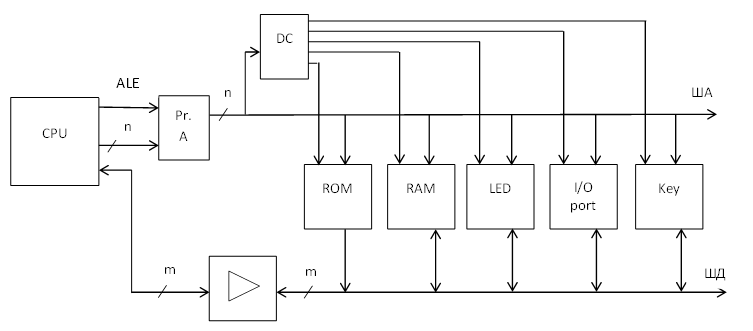
\includegraphics[width=0.8\textwidth]{101_struct.png}
\end{figure}

Допустим шина адреса процессора включает 16 бит, а шина данных ---- 8 бит, тогда максимальный объем адресуемой памяти составит 64 Кбайт. Предположим, что для ОЗУ необходимо выделить 32 Кбайта, ПЗУ -- 8 Кбайт, индикация ---- 256 байт, порт ввода/вывода ---- 256 байт, клавиатура ---- 256 байт, регистры процессора 4 -- Кбайт. При делении адресного пространства между блоками необходимо соблюдать, чтобы начальный адрес каждого блока начинался с нулей, а старший заканчивался на “F”.

В адресном пространстве каждый из блоков будет иметь следующие значения:

$
\begin{array}{lll}
\text{ОЗУ:} & \text{ПЗУ:} & \text{Индикация, порт, клавиатура по:}\\
\underbrace{1000}_{\mbox{8}}
\underbrace{0000}_{\mbox{0}}
\underbrace{0000}_{\mbox{0}}
\underbrace{0000}_{\mbox{0 h}}&
\underbrace{0010}_{\mbox{2}}
\underbrace{0000}_{\mbox{0}}
\underbrace{0000}_{\mbox{0}}
\underbrace{0000}_{\mbox{0 h}}&
\underbrace{0000}_{\mbox{0}}
\underbrace{0000}_{\mbox{0}}
\underbrace{1111}_{\mbox{F}}
\underbrace{1111}_{\mbox{F h}}\\
\\
\text{Регистры процессора:}\\
\underbrace{0001}_{\mbox{1}}
\underbrace{0000}_{\mbox{0}}
\underbrace{0000}_{\mbox{0}}
\underbrace{0000}_{\mbox{0 h}} 
\end{array}
$

\begin{center}
\begin{tabular}{|c|c|c|}
\hline 4000h --- BFFFh & ОЗУ                 &  32 Кбайт  \\
\hline 3200h --- 32FFh & порт ввода/вывода   &  256 байт  \\
\hline 3100h --- 31FFh & клавиатура          & 256 байт   \\
\hline 3000h --- 30FFh & индикация           & 256 байт   \\
\hline 1000h --- 2FFFh & ПЗУ                 &  8 Кбайт   \\
\hline 0000h --- 0FFFh & регистры процессора & 4 Кбайт    \\
\hline
\end{tabular}
\end{center} 

% Вопрос 102 ---------------------------------------------------------------------------------------------------------------
\section{Укажите место на структурной схеме ЭВМ различных интерфейсов. Как объединять ЭВМ в  систему? Какие условия следует выполнить при  передаче данных? Обоснуйте.}

\begin{figure}[H]
\centering
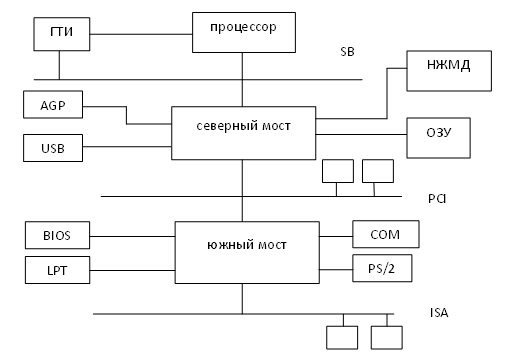
\includegraphics[width=0.8\textwidth]{./images/102_interface.png}
\end{figure}

В структуре ЭВМ в зависимости от назначения используются следующие интерфейсы:
\begin{enumerate}
\item Межпроцессорные интерфейсы --- для объединения нескольких процессоров: шинный интерфейс с адресным арбитражем(по командам).
\item Межсистемный интерфейс --- для объединения нескольких вычислительных блоков в одну систему. Задача возникает в кластерах. Необходим быстрый коммутатор и сеть типа 1 Гбит.
\item Системные интерфейсы --- набор шин с правилами обмена между основными блоками ЭВМ(LS, SB, PCI, ISA).
\item Интерфейсы ВУ (периферийные) --- обмен информации между системным блоком и ВУ (COM, USB, LPT, PS/2).
\end{enumerate}

При проектировании и реализации схемы интерфейса необходимо выполнить три условия согласования для передачи от устройства к приемнику:
\begin{enumerate}
\item Механические
\item Логические
\item Электрические
\end{enumerate}

Механические --- тип разъема, число контактов, расстояние между ними.

Логические --- последовательность передачи сигналов и наличие сигналов синхронизации определяется протоколом интерфейса, форматом передаваемого кадра и в конечном счете программным управлением. Уровни <<1>> и <<0>> так же определяются логическими условиями.

Электрические --- временные положения импульсов, величина фронтов, длительность сигналов синхронизации, фазовые сдвиги.

Помимо условий согласования необходимо выполнить интерфейсные функции: на время в буфере сохранить сигнал, проанализировать ответный сигнал, сформировать сигнал сопровождения и т.д.

% Вопрос 103 ---------------------------------------------------------------------------------------------------------------
\section{Расставьте по убыванию значимости параметры ЭВМ по критерию производительности. Охарактеризуйте эти параметры.}

Производительность --- число операций выполняемых в единицу времени. Если данные представлены в целом коде --- единица измерения MIPS (миллион инструкций в секунду). Если данные представлены в  формате ПЗ --- единица измерения FLOP (операций в секунду). Производительность комьютера не вычислияется, а определяется в процессе тестирования по скорости выполения определенных операций в программной среде.
Параметры влияющие на производительность ЭВМ:
\begin{enumerate}
\item Одно- или многопроцессорная система
\item Значение тактовой частоты
\item Разрядность шины адреса и данных
\item Интерфейсы
\end{enumerate}

Производительность в первую очередь зависит от типа вычислительной системы. Многопроцессорность позволяет увеличить производительность ЭВМ, так как выполняет множество параллельных программных процессов в системе.

Такт --- это интервал времени, затрачиваемый на выполнение одной простейшей машинной операции. Следовательно, тактовая частота --- это количество тактов в секунду. Один такт в секунду равен одному Герцу. Современные компьютеры работают на тактовых частотах в несколько сотен Мегагерц, т.е. выполняют несколько десятков или сотен миллионов простейших машинных операций за одну секунду. Поэтому с увеличением частоты тактируемых импульсов растет быстродействие, а с ней и производительность ЭВМ.

Разрядность шины адреса и данных --- определяет количество бит передаваемых шиной. Чем больше разрядность, тем большее количество информации можно передать за один такт.

Периферийные нтерфейсы. Типы системного и локальных интерфейсов. Разные типы интерфейсов обеспечивают разные скорости передачи информации между узлами машины, позволяют подключать разное количество внешних устройств и различные их виды. 

% Вопрос 104 ---------------------------------------------------------------------------------------------------------------
\section{Преобразуйте десятичное число в различные форматы хранения. В какой форме хранятся в памяти ЭВМ символы. Приведите два примера.}

Методика преобразования целых десятичных чисел в двоичные коды различна в зависимости от знака числа.

Положительные числа имеют одинаковое представление в обратном, прямом и дополнительном кодах, и имеют цифру $ 0$ в знаковом разряде: $127_{10}=01111111_{2}$.

Отрицательные числа представляются в виде дополнительного кода. Преобразование из прямого кода в дополнительный сводится к следующим действиям:
\begin{enumerate}
\item Прямой код

В знаковый разряд помещается цифра $ 1 $, а в разряды цифровой части числа --- двоичный код абсолютной величины: $-127_{10}=11111111_{2}$
\item Обратный код

Получается инвертированием всех цифр двоичного кода без учета знакового разряда: нули заменяются единицами и наоборот: $-127_{10}=10000000_{2}$
\item Дополнительный код

К обратному коду добавляется единица к младшему разряду: $-127_{10}=10000001_{2}$.
Дополнительный код и есть представление отрицательного числа $-127$.
\end{enumerate}  

Преобразование вещественных чисел со знаком:

Вещественное число {\it X} можно представить в виде произведения мантиссы {\it m } и основания системы счисления {\it q } в некоторой степени {\it n } : $ X=m \ast q^{n} $. 
Например: $ 25.324 = 0.25324\ast 10^{2} $. Здесь $ 0.25324 $ --- мантисса в нормальной форме, $ 2 $ --- порядок(степень). Порядок указывает, на какое количество позиций должна сместиться запятая в мантиссе. Необходимо, чтобы значение мантиссы было удовлетворяло условию: $ 0.5 \leq m < 1 $. Другими словами нормализованная мантисса меньше $ 1 $ и первая значащая цифра после запятой не меньше $ 5 $. 
Двоичный код вещественного числа должен быть следующего формата:

\begin{center}
\begin{tabular}{|c|c|c|}
\hline 8 бит   & 1 бит & 23 бит   \\ 
\hline порядок & знак  & мантисса \\ 
\hline 
\end{tabular}
\end{center}
 
Допустим имеем число $278.15$, переведем его в двоичный код в формате п.з.. Подставим это число в формулу $ X=m\ast q^{n} $. Получим уравнение:$278.15= m\ast q^{n}$. Для нахождения мантиссы $m$ неизвестен порядок $n $, найдем его: $2^{8}=256$, что меньше $278.15$, возьмем следующую степень по порядку $-2^{9}=512$. В данном случае $512>278.15$, по этому выберем $q^{n}=2^{9}$. Тогда мантисса $m=X/q^{n} =278.15/512=0.543$. Прямой код мантиссы $m=0.543=10001_{2}$. Прямой код порядка $n=9=1001_{2}$. Теперь можно записать число в формате с плавающей запятой:

\begin{center}
\begin{tabular}{|c|c|c|}
\hline порядок  & знак & мантисса                \\ 
\hline 00001001 & 0    & 10001000000000000000000 \\ 
\hline 
\end{tabular}
\end{center}

Преобразование в шестнадцатеричные коды:

Преобразование из двоичного кода в шестнадцатеричный производят в два этапа: перевод в двоичный код, а затем уже в шестнадцатеричный.

Для преобразования из двоичного кода в шестнадцатеричный нужно условно разбить код на тетрады. Например, необходимо преобразовать код: $ 110100011,1111_{2} $. Разбиваем его на тетрады: $ 1 \mid 1010 \mid 0011 \mid 1111 $. И каждую тетраду заменяем на соответствующее шестнадцатеричное число. $ 1_{2} = 1_{16} $, $ 1010_{2} = A_{16} $, $ 0011_{2} = 3_{16} $, $ 1111_{2} = F_{16} $. В итоге получим число $ 1A3,F $. В таблице указано соответствие двоичных чисел шестнадцатеричным:

\begin{center}
\small
\begin{tabular}{|c|c|c|c|c|c|c|c|c|c|c|c|c|c|c|c|}
\hline 0000 & 0001 & 0010 & 0011 & 0100 & 0101 & 0110 & 0111 & 1000 & 1001 & 1010 & 1011 & 1100 & 1101 & 1110 & 1111 \\ 
\hline 0 & 1 & 2 & 3 & 4 & 5 & 6 & 7 & 8 & 9 & A & B & C & D & E & F \\ 
\hline 
\end{tabular}
\end{center}

Преобразование в двоично-десятичный код:

Преобразование десятичного числа в двоично-десятичный код осуществляется переводом каждого разряда десятичного числа в соответствующий четырехбитовый эквивалент. Например, число $ 311_{10} = 011100010001_{BCD} $. Здесь  $3_{10} = 0111_{2}$, $1_{10} = 0001_{2}$.

Хранение символов в ЭВМ:

Каждая буква принадлежит определенному алфавиту, в котором символы следуют друг за другом и, следовательно, могут быть пронумерованы последовательными целыми числами. Каждой букве можно сопоставить целое положительное число и назвать его кодом символа. Именно этот код будет храниться в памяти компьютера, а при выводе на экран или бумагу «преобразовываться» в соответствующий ему символ. Чтобы отличить представление чисел от представления символов в памяти компьютера, приходится также хранить информацию о том, какие именно данные закодированы в конкретной области памяти.

Соответствие букв определенного алфавита с числами-кодами формирует так называемую таблицу кодирования. Другими словами, каждый символ конкретного алфавита имеет свой числовой код в соответствии с определенной таблицей кодирования. Американским национальным институтом стандартизации (ANSI) была разработана таблица кодирования символов, которая впоследствии была использована во всех операционных системах. Эта таблица называется ASCII.

Например, символу $A$ соответсвует код 41h, а символу $+$ код 2Bh. 

% Вопрос 105 ---------------------------------------------------------------------------------------------------------------
\section{Сопоставьте принципы печати лазерного и струйного принтеров, опишите и сравните их.}

{\bf Лазерный принтер:}

В основе печати лазерным способом лежит принцип переноса изображения из кодов на образующую фотобарабана лазерным лучом. Луч двигается слева направо(принцип монитора) при этом модулируется так же знакогенераторм или графическим процессором, барабан перемещается всякий раз на одну линию и далее уже красящее вещество с барабана механически переносится на бумагу. Печатающий узел называется катридж. Основа в катридже --- кожух с продольным отверстием, которое закрывается шторкой. При сдвиге шторки через отверстие виден барабан светлого света, покрытый селеном потому, что он под воздействием света проявляет внешний фотоэлектрический эффект. Помимо барабана в кожухе размещается красящий порошок --- тонер --- мелкодисперсный синтетический состав, плавящийся при нагревании. С торцов катриджа система шестерен для управления вращением барабана. Так же в катридже расположен электрод, на который подается высокое отрицательное напряжение. Коды символов, поступая в процессор принтера преобразовываются в управляющую 
последовательность кодов. Эта последовательность единиц и нулей посылается на лазер --- источник света с тонким лучом. Луч направлен на зеркало, которое перемещает его строго по образующей барабана с одного конца на другой. Подавая 1 и 0 на лазер, формируются светлые и темные точки на образующей цилиндра.
\begin{figure}[H]
\centering
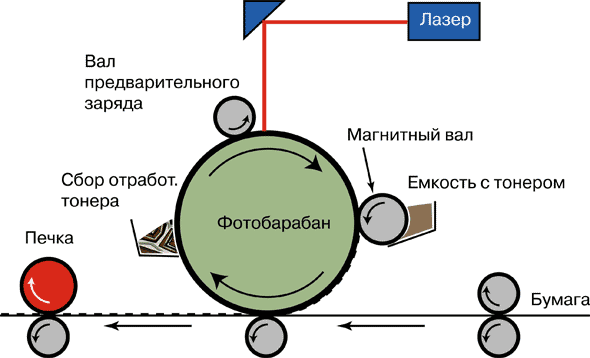
\includegraphics[width=0.6\textwidth]{105_Laser.png}
\caption{Лазерный принтер}
\end{figure}
В начальном состоянии барабан не заряжен, тонера на нем нет. Но рядом с барабаном имеется электрод, заряжающий барабан отрицательно. При вращении барабана его поверхность заряжается равномерно. При печати луч лазера попадает через зеркало на образующую барабана и выбивает электроны в том месте куда он попал. После того как пройдет развертка, формируются заряженные и незаряженные точечки. При дальнейшем движении сверху сыплется порошок, имеющий отрицательный заряд. При соприкосновении с поверхностью цилиндра порошок прилипает к его незаряженным частям. Барабан вращается дальше, и в нижней точке соприкасается с листом бумаги, образуя оттиск на бумаге --- барабан вдавливается в бумагу. Бумага двигается далее по роликам нагревается, и, порошок расплавляясь, въедается в бумагу. Поскольку развертка движется периодически, на поверхности барабана получаем рисунок, символы в котором непрерывным путем переносятся на бумагу.

Преимущество: скорость печатания лазерных принтеров велика --- до нескольких десятков страниц в минуту. Разрешающая способность 300-1200 dpi. Являются экономичными.

Недостаток: один тонер. Поэтому для цветной печати выполняют три пишущих узла, с разными тонерами (RGB). Цвета наносятся друг за другом  и затем сплавляются. 

{\bf Струйный принтер:}

Развитием в сторону бесконтактного способа матричной печати (иголок), является печать капельками жидкости --- струйные принтеры. У таких принтеров капельки красящего вещества выстреливают из сопла головки, пролетают небольшое расстояние и попадают на бумагу. Основная проблема в таких устройствах печати --- это то, как "прилепить" каплю жидкости к бумаге. В струйных принтерах бумага должна быть не очень плотной, и в то же время иметь плотность не хуже некоторого значения, по скольку жидкость распространяется во все стороны. Задача решается совместно: определенное качество бумаги и текучести чернил. По скольку капелька вытекает из сопла, то можно размещая по три сопла рядом печатать цветом. На практике существуют два способа струйной печати: {\sl Непрерывная и импульсная струйная печать.}

{\it Непрерывная струйная  печать:}

Чернила подаются в печатающую головку с помощью насоса. Возникающая под создаваемым им давлением струя разбивается на капельки за счет вибрации, вызываемой, например, пьезоэлектрическим элементом. Разумеется, до бумаги должны долететь не все, а только часть капелек, иначе никакого изображения не получится --- бумага просто будет равномерно залита чернилами.
Вылетая из сопла, капельки проскакивают через заряжающий электрод. Получив электрический заряд, они попадают в поле отклоняющего электрода, на который подается высокое напряжение. Изменяя напряжение на отклоняющем электроде, можно заставить капельки поменять траекторию полета. Если состоящая из заряженных капелек струя не отклоняется в сторону, она попадает в уловитель, из которого неиспользованные чернила стекают в накопитель, проходят стадию удаления воздушных пузырьков (дегазации) и снова сливаются в основной резервуар с краской.
Сменившие направление полета под действием электрического поля отклоняющего электрода капельки попадают на бумагу, формируя на ней изображение. Угол отклонения траектории зависит от того, насколько сильно изменяется напряжение.
Системы непрерывной струйной печати отличаются тем, что в них применяется дорогая электропроводная краска, способная получить заряд. Так как между соплом и бумагой необходимо разместить два электрода, увеличивается дальность полета капелек и, следовательно, им необходимо придать большую начальную скорость. Очень высока и производительность сопел печатающей головки --- из них в секунду вылетает от 50 до 150 тысяч капелек. Однако сам процесс печати не назовешь очень быстрым.

Недостаток: медленная печать, серьезные эксплуатационные расходы, обусловленные дороговизной чернил и сложностью обслуживания таких принтеров, и, конечно, немалая цена самого оборудования.

Преимущество: высокое качество получаемых с ее помощью цветных изображений.

{\it Импульсная струйная печать:}

Капельки из сопел пьезоэлектрической головки вылетают под воздействием создаваемого на очень короткое время избыточного давления в камере с чернилами. Для образования в камере избыточного давления применяется диск из пьезоэлектрика. Когда к нему подводится напряжение, он деформируется (изгибается). Выгнувшись, диск, который служит одной из стенок камеры с чернилами, резко уменьшает ее объем, оказавшиеся лишними чернила вылетают при этом из сопла в виде капельки. Для заполнения камеры, когда напряжение снято и пьезоэлектрический диск возвращается к исходной форме, применяется капиллярный способ подачи чернил из резервуара. 

\begin{figure}[H]
\centering
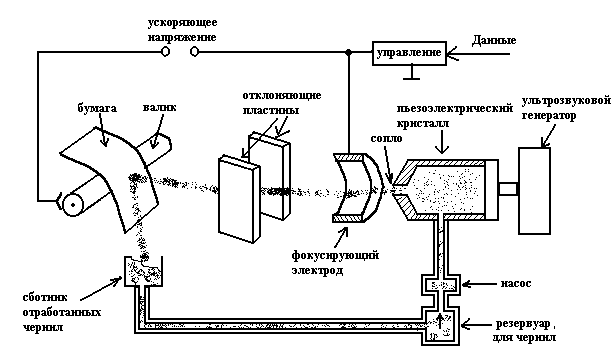
\includegraphics[width=0.6\textwidth]{105_Strui.png}
\caption{Струйный принтер на основе пьезоэлектрика }
\end{figure}

Конструкция современных пузырьковых головок допускает использование быстро сохнущих чернил, благодаря чему капельки не успевают впитаться в бумагу или растечься --- они просто моментально высыхают. Благодаря увеличению скорости, с которой из сопел выстреливаются капельки, можно увеличить зазор между головкой и бумагой. Больший зазор позволяет применять бумагу худшего качества, неровную или более плотную.Такая технология привела к упрощению конструкции, удешевлению самих принтеров, так и к снижению эксплуатационных затрат.

\section{Приведите две схемы подключения клавиатуры к портам ввода-вывода. Приведите алгоритм опроса пассивной матричной клавиатуры.}

% Вопрос 106 ---------------------------------------------------------------------------------------------------------------
Схема подключения клавиатуры через регистр с прерыванием:

Тактовый сигнал непрерывно пишет в регистр состояние кнопок, в то время как $cs$ пока не открывает выход. По нажатию кнопки, сигнал прерывания поступает в процессор, который запускает подпрограмму обработки клавиатуры. Процессор выставляет адрес закрепленный за клавиатурой, адресный дешифратор формирует $cs$, и на выходе регистра появляется состояние кнопок. Сигналы с выхода регистра поступают в какой либо внутренний регистр процессора, определяется один или несколько активных разрядов и соответствующая кнопка. 

\begin{figure}[H]
\centering
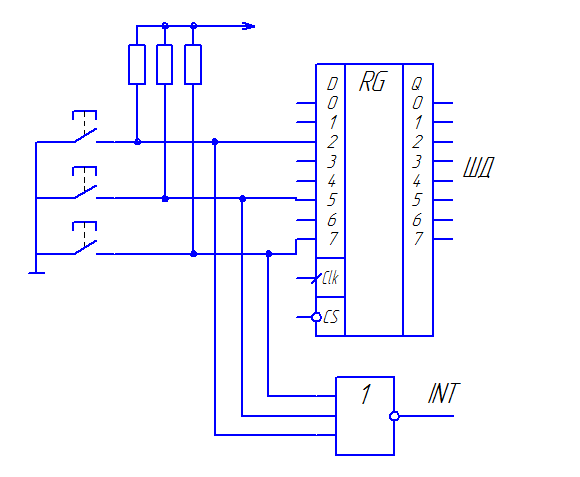
\includegraphics[width=0.4\textwidth]{106_Button.png}
\caption{Подключение кнопок через регистр с прерыванием}
\end{figure}

Схема подключения матричной клавиатуры

Пассивная матрица $4\times 3$ имеет 4 строки и 3 столбца. На пересечении столбец/строка стоит кнопка, не обязательно гальванический контакт, возможен емкостный.

По каналу {\it А} в порт отправляем из процессора сканирующий код следующей структуры: {\it 1110, 1101, 1011, 0111}. Выставив первый код, мы читаем по каналу {\it В} состояние разрядов. При появлении 0 на {\it A0} и замыкании верхнего ключа, разряд {\it B0} становится низким по скольку ток с контакта {\it +5B} течет через резистор и диод на {\it A0}. Читая код по {\it B} определяем есть ли в нем 0 и в каком разряде. Если в возбужденной строке появился 0 значит одна из трех кнопок в возбужденной строке замкнута, осталось определить которая. Чтобы определить которая кнопка замкнута необходимо последовательно маскировать каждый из разрядов порта {\it B}. Конкретный разряд умножаем на 1 а другие на 0 и смотрим 1 или 0 в данном разряде. Если 0 то через таблицу присвоения символа определяем какая нажата, выполняя подпрограмму. Сочетание активной строки и 0 в принятом столбце дает указанную кнопку.

\begin{figure}[H]
\centering
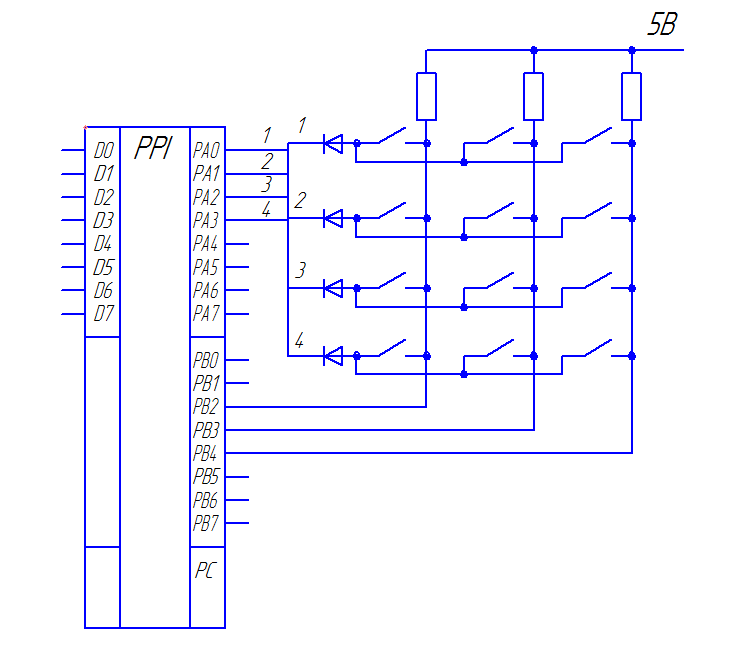
\includegraphics[width=0.4\textwidth]{106_Keyboard.png}
\caption{Матричная клавиатура}
\end{figure}

% Вопрос 107 ---------------------------------------------------------------------------------------------------------------
\section{Выберите способ обмена данными между процессором и внешним устройством. Обоснуйте выбор. Напишите процедуру ввода или вывода данных в память ЭВМ в мнемонике команд (уровень ассемблера).}

Задача обмена данными между внешним устройством и процессором сводится к пересылке данных между памятью внешнего устройства(ВУ) и памятью ОЗУ. Существует 3 подхода к обмену информации между процессором и ВУ: программный обмен, ввод/вывод с отображением в память, прямой доступ к памяти (ПДП). Из этих способов предпочтительней является ПДП.

ПДП отличается от предыдущих методов тем, что не задействует процессор при обмене информацией. Функцию процессора на время обмена данными ВУ-ОЗУ выполняет контроллер ПДП. Контроллер представляет собой небольшой автомат, имеющий внутренний счетчик с начальным установом и логику проверки конца счета. 

Последовательность работы заключается в следующем:

Программа формирует сигналы прерывания процессору. Программное прерывание служит сигналом процессору и тот переводит выводы в третье состояние. Если же ввод идет по инициативе внешнего устройства, то ВУ посылает прерывание на процессор. Может быть так что ВУ посылает запрос на контроллер ПДП, который формирует прерывание на процессор. 

Процессор переводит выходные разряды в третье состояние, но перед этим посылает по адресу ПДП по шине данных режим работы и начальный адрес массива памяти, объем, либо конечный адрес. Эти три величины пишутся в контроллере и настраивают его на направление и начальный адрес. После перевода шин в третье состояние, контроллер выставляет начальный адрес на шину адреса, сигнал управления, и выводы внешнего устройства напрямую подключаются к шине данных. Цикл обмена по времени занимает 1 такт работы процессора --- скорость обмена максимальная. Обмен производится до тех пор пока не отработает последний адрес. После чего контроллер посылает на процессор сигнал отмены прерывания. Процессор продолжает работу.

\begin{figure}[H]
\centering
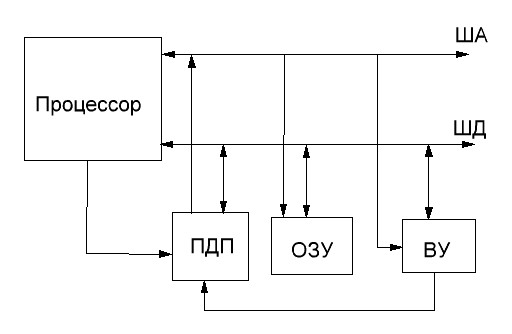
\includegraphics[width=0.4\textwidth]{107_PDP.JPG}
\caption{Ввод/вывод с контроллером ПДП}
\end{figure}  

Процедура ввода данных в память ЭВМ:

\begin{center}
\begin{tabular}{l l}
    & {} M100          \\ 
101 & {} MVI E, 00h    \\ 
102 & {} LXI H, 0020h \\ 
103 & {} MOV M, E      \\ 
104 & {} INR E         \\ 
105 & {} INX H        \\ 
106 & {} MOV A, E      \\ 
107 & {} CPI 81h       \\ 
108 & {} JZ 103        \\  
\end{tabular} 
\end{center}

Процедура последовательно вводит в память начиная с адреса {\sl 2000h} числа от {\sl 00h} до {\sl 80h}. По команде {\sl MVI E}, в регистр {\sl E} записывается число {\sl 00h}. Начальный адрес ячейки памяти {\sl 2000h} копируется с помощью команды {\it LXI} в регистр {\it HL}. По скольку первый байт операнда записывается в регистр {\sl L}, а второй --- в регистр {\sl H}, мы записали этот операнд в виде {\sl 0020h}. Используя {\sl MOV M}, копируется число из региcтра {\sl E} в ячейку памяти, адрес которой содержится в регистре {\sl HL}. Чтобы записать следующее число в следующую ячейку памяти, производим опреацию инкрементирования. По команде {\sl JZ} каждый раз происходит переход на операцию ввода данных в ячейку памяти {\sl MVI E}, но только до тех пор пока не запишется последнее число {\sl 80h}. Благодаря команде {\sl CPI} можно проверить конец вводимых в память значений. Число {\sl 81h} не запишется в память, так как по команде {\sl CPI} выставится флаг нуля и не произойдет перехода на строку с командой 
записи в память.

% Вопрос 108 --------------------------------------------------------
\section{Приведите основные архитектурные варианта построения операционных систем. Поясните понятие <<виртуальная машина>>.}
\begin{enumerate}
\item Монолитные системы (монолитное ядро, monolithic kernel) --- представляет собой простейшую структуру, когда компоненты операционной системы являются не самостоятельными модулями, а составными частями одной программы. Операционная система написана в виде набора процедур.
\item Многоуровневые системы --- является организация операционных систем в виде иерархии уровней.
\item Виртуальные машины.
\item Экзоядро --- реализован принцип обеспечения каждого пользователя абсолютной копией реального компьютера, но с подмножеством ресурсов. На нижнем уровне в режиме ядра работает программа --- экзоядро (exokernel), в задачу которой входит распределение ресурсов для виртуальных машин и проверка их использования (отслеживание попыток машин использовать чужой ресурс).
\item Ядро в привилегированном режиме --- Операционная система должна иметь по отношению к приложениям определенные привилегии, иначе некорректно работающее приложение может вмешаться в работу операционной системы и разрушить часть ее кодов. Аппаратура компьютера должна поддерживать как минимум два режима работы --- пользовательский (user mode) и привилегированный (режим ядра, kernel mode или режим супервизора, supervisor mode). Так как ядро выполняет все основные функции операционной системы, то чаще всего именно оно работает в привилегированном режиме.
\item Многослойная структура операционной системы --- вычислительная система, работающяя под управлением операционной системы на основе ядра, можно рассматривать как систему, состоящую из трех иерархически расположенных слоев: нижний слой образует аппаратура, промежуточный --- ядро, верхний --- утилиты, обрабатывающие программы и приложения. При такой организации приложения не могут непосредственно взаимодействовать с аппаратурой, а только через слой ядра.
\item Микроядерная архитектура  ---  большинство составляющих операционной системы являются самостоятельными программами Взаимодействие между программами операционной системы обеспечивает специальный модуль ядра --- микроядро. Микроядро работает в привилегированном режиме и обеспечивает взаимодействие между программами, планирование использования процессора, первичную обработку прерываний, операции ввода-вывода и базовое управление памятью. Остальные компоненты системы взаимодействуют друг с другом путем передачи сообщений через микроядро.
\item Модель клиент-сервер --- операционные системы в кторых происходит перенос большинства задач на операционной системы на средства пользовательских процессов.
\item Смешанные системы --- операционные системы использующие различные комбинации перечисленных подходов.
\end{enumerate}

Виртуальная машина --- это вычислительная среда, набор ресурсов и правил работы которой формируется (с помощью программного обеспечения) в некой другой вычислительной среде.


% Вопрос 109 --------------------------------------------------------
\section{Спроектировать устройство управления программного типа. Число микрокоманд в цикле --- не более 7. Привести примеры циклов: выборка команды, чтение памяти и запись в память. Чем определяется период следования тактового сигнала.}

Распространены в CPU с командным управлением. С выхода регистра микрокоманд часть разрядов возвращается на дешифратор --- это обратная связь. Цепь разделена регистром и соответственно изменяет состояние по тактовому сигналу «С». Поэтому если в обратной связи 3 разряда, то на двух разрядах вернувшихся на вход дешифратора возможны 8 комбинации. Т.е. из одного КОП мы можем сделать 4 комбинации микрокоманд. Основной блок устройства дешифратор имеет жесткие связи (пайка, металл на ИМС), поэтому изменить микрокоды возможно только если заменить схему на новую. Предлагалось сделать дешифратор на основе программируемой матрицы. Мы запрограммировали матрицу --- получили свои микрокоды. Где-то эти микрокоды нас не устроили. Мы можем перепрограммировать этот дешифратор и получить новые микрокоды. Микрокоды считаются секретными, поскольку именно от них зависит время выполнения команды. На практике дешифраторы размещают на кристалле процессора и настраивают (программируют) металлом, выполняя соединение в матрице. В тех 
случаях, когда время выполнения команд должно быть строго фиксировано лучше применять микропрограммный способ управления.
 
\begin{center}
\begin{figure}[H]
\centering
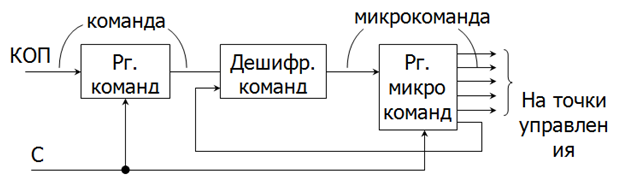
\includegraphics[width=0.6\textwidth]{109_struct.png}
\caption{Структура устройства программного управления}
\end{figure}  
\end{center}

% Вопрос 110 --------------------------------------------------------
\section{Спроектировать устройство микропрограммного управления автономного типа. Источник управляющих кодов --- счетчик микрокоманд, число состояний счетчика --- 32. Разрядность регистра микрокоманд --- 24.}

Счетчик микрокоманд, имеющий 5 выводов на выходе, позволяет производить выборку из МПЗУ 32 команд. По выбранному адресу, команда поступает по 24 разрядной шине из МПЗУ в регистр микрокоманд. Устройство автономное и имеет генерато ртактовых импульсов.

\begin{center}
\begin{figure}[H]
\centering
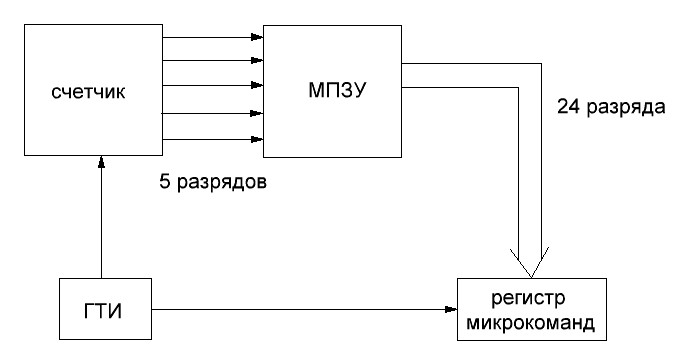
\includegraphics[width=0.6\textwidth]{110_struct.JPG}
\caption{Структура устройства микропрограммного управления}
\end{figure}  
\end{center}

%Вопрос №111-------------------------------------------------------------------------------------
\section{Привести примеры процедур с различными способами адресации для пересылки содержимого ячейки памяти команд в ячейку памяти данных в мнемонике команд, адресация в пределах одной страницы (64 кб). Пояснить необходимость модификации адресов для доступа к данным и возможные их способы.}

В памяти команд лежат константы, которые понадобятся в дальнейшем выполнении программы.\\
MVI A,3E\\
STA 12ED\\
В данном примере байт константы (3Е) записывается сначала в аккумулятор процессора, а затем из него в ячейку памяти по адресу 12ED.

Команда MVI A,(d8) -- непосредственная адресация, записывает константу, расположенную в памяти команд  следующей после КОП.
%однострочная аблица с КОП
\begin{center}
\begin{tabular}{|c|c|}
\hline КОП  & data 8 бит \\  
\hline 
\end{tabular}
\end{center}
Команда STA -- \underline{прямая адресация}, записывает значение аккумулятора по адресу указанному в следующих 2 байтах после КОП.
\begin{center}
\begin{tabular}{|c|c|}
\hline КОП & адрес 16 бит \\ 
\hline 
\end{tabular}
\end{center}
MVI A,7C\\ 
STAX B\\
В этом примере байт константы (7С) записывается сначала в аккумулятор процессора, а затем из него в ячейку памяти по адресу расположенному в регистровой паре ВС.

Команда STAX B -- \underline{косвенная адресация}, записывает в ячейку памяти данных значение аккумулятора, по адресу, расположенному в регистрах ВС.
\begin{center}
\begin{tabular}{|c|}
\hline КОП \\ 
\hline 
\end{tabular}
\end{center}
MVI M,43\\
MVI M -- команда \underline{непосредственно-косвенной адресации}, когда константа , лежащая в памяти команд записывается в ячейку памяти данных.
\begin{center}
\begin{tabular}{|c|c|}
\hline КОП & data 8 бит \\ 
\hline 
\end{tabular}
\end{center}

Модификации адресов произошла в следствии увеличения объема адресуемой памяти. Всю память поделили на страницы фиксированной длинны и для её адресации используются новые методы.

\underline{Страничная адресация} -- адрес получается путем присоединения значения ячейки в странице к номеру страницы. adr = l.m

\begin{figure}[H]
\centering
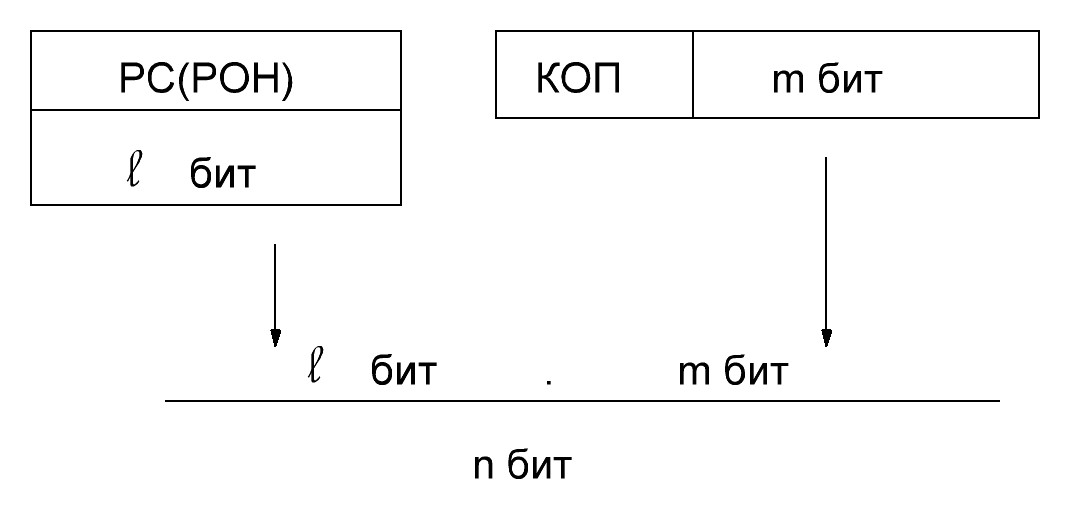
\includegraphics[width=0.6\textwidth]{111_Stranichna.JPG}
\caption{Получение физического адреса}
\end{figure}
При ША равной n бит , n= l + m , где l бит-номер страницы, а m бит-ячейка в странице.

Номер страницы хранится в специальном регистре, так же он может быть и в РОН, а номер ячейки указывается в адресном поле команды.
Страничная адресация имеет следующие достоинства:
\begin{enumerate}
\item Перемещаемость программ и данных обеспечивается путем занесения номера текущей страницы в регистр номера страницы.
\item Длина поля ячейки страницы небольшая и постоянная m < n.
\item Расширение адресного пространства при небольшом адресном поле в команде.
\end{enumerate}
Недостатки страничной адресации:
\begin{enumerate}
\item Сложности с организацией переходов в программе за пределы страницы, нужно изменять содержимое регистра номера страницы, что приводит к снижению быстродействия.
\item не эффективное использование памяти , т.к. распределение между задачами происходит постранично, поэтому часть последней страницы может пустовать. 
\end{enumerate}

\underline{Относительная адресация} -- образует адрес путем смещения относительно начала страницы. Физический адрес получается при сложении значения  смещения, находящегося в поле адреса команды, и значения базового  адреса, находящегося в базовом регистре процессора.\\
adr(n бит) = B(n бит) + D(n бит), где В --- значение базового адреса(начало страницы), D --- значение смещения.

Страничная адресация является частным случаем относительной. 
\begin{figure}[H]
\centering
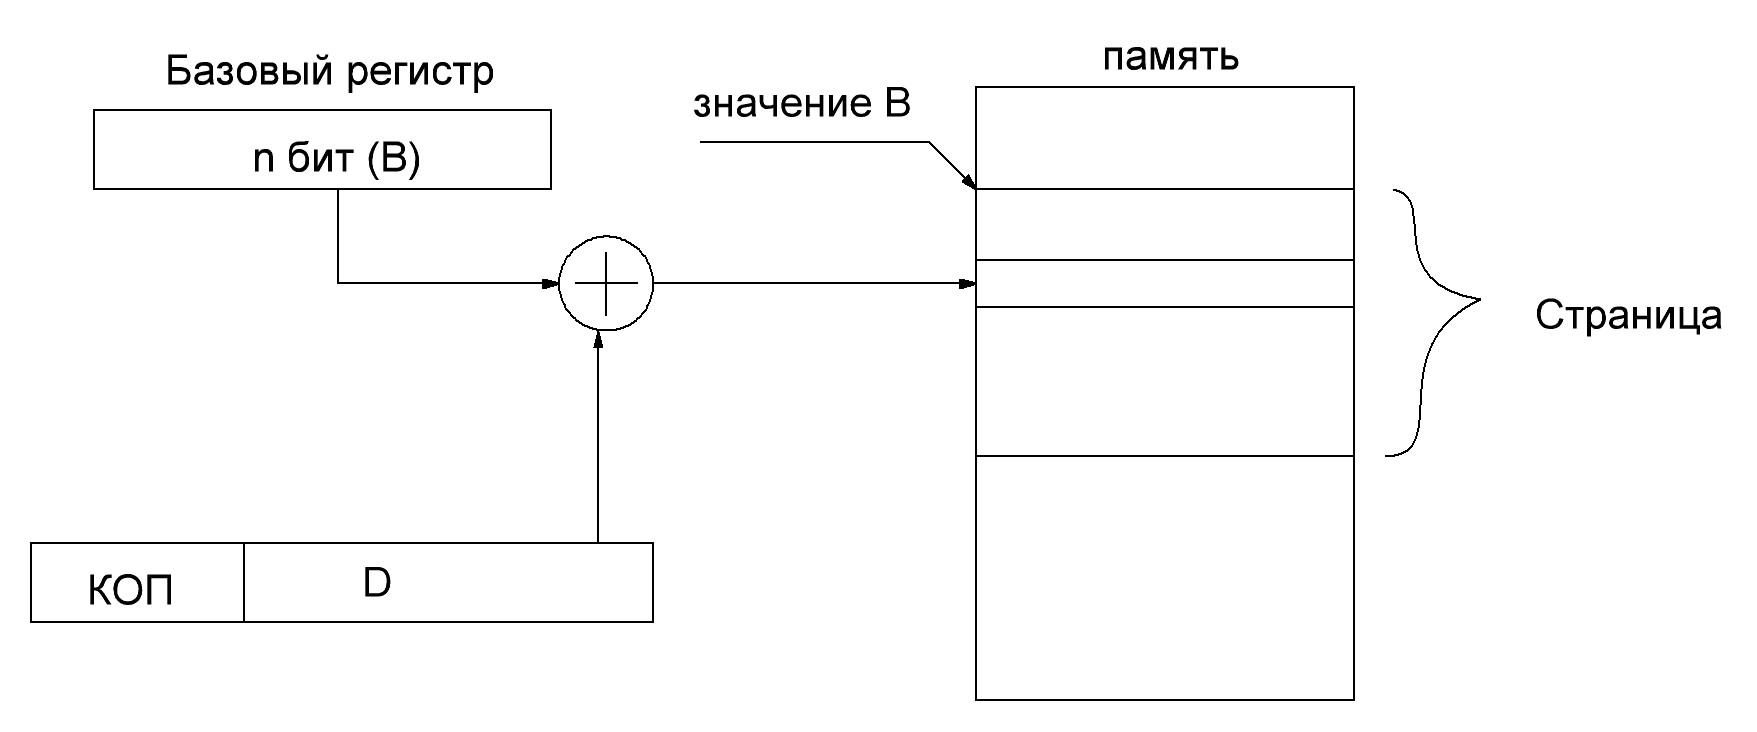
\includegraphics[width=0.6\textwidth]{111_Otnositelna.JPG}
\caption{Получение физического адреса}
\end{figure}


\underline{Индексная адресация} -- используется для адресации элементов массивов. Физический адрес получают путем сложения значения базового адреса, находящегося в поле адреса команды, и значения индексного регистра.

\begin{figure}[H]
\centering
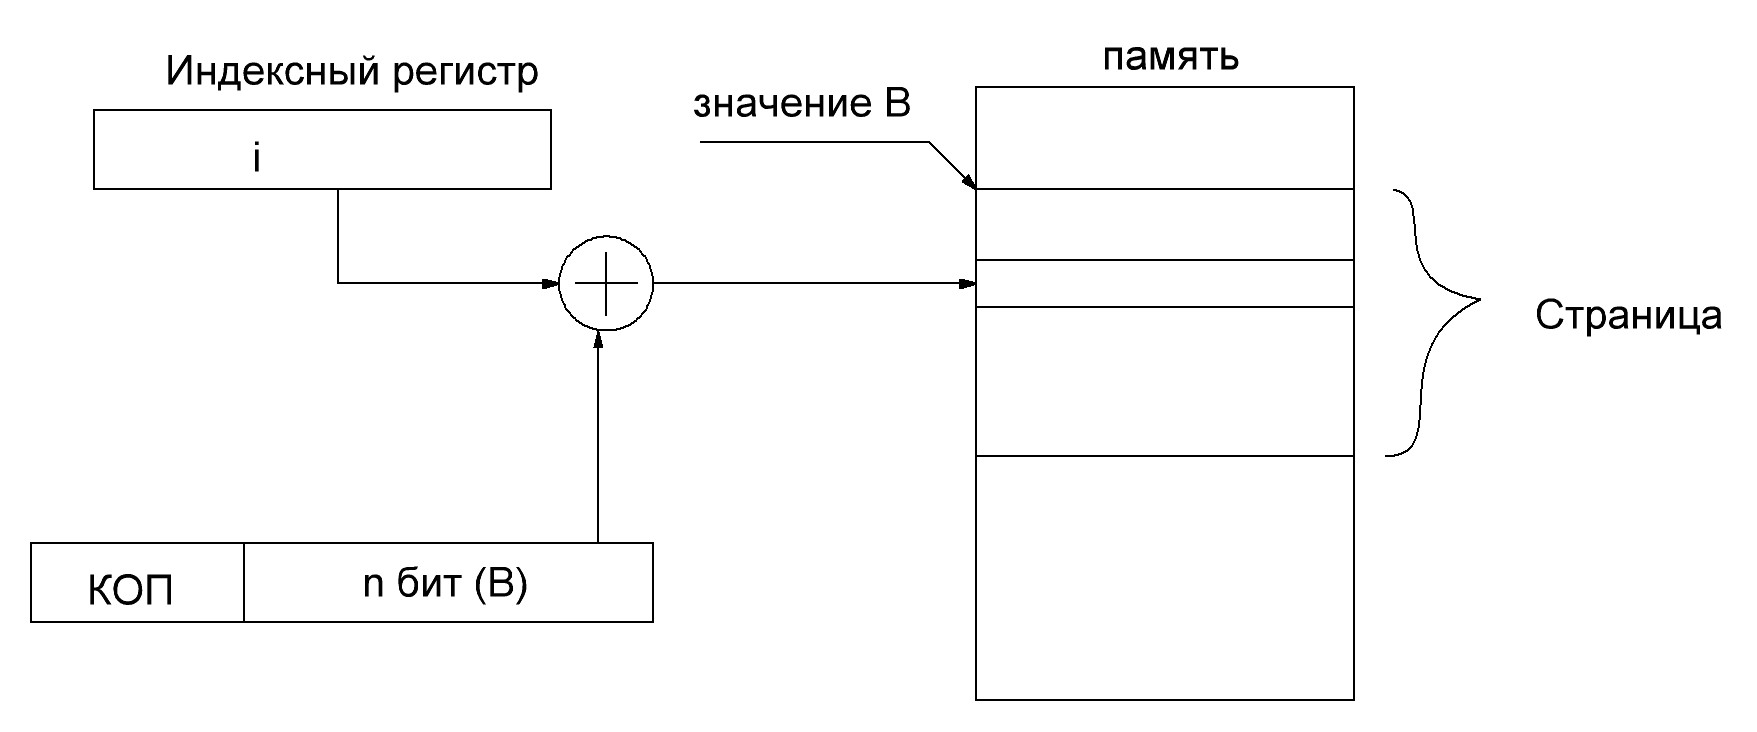
\includegraphics[width=0.6\textwidth]{111_Indexna.JPG}
\caption{Получение физического адреса}
\end{figure} 
\underline{Индексно-относительная адресация} -- совместное использование индексной и относительной адресации. 
adr = i + B + D, где i-индекс, В-базовый адрес, D-смещение.

Все модифицированные способы адресации направлены на формирование адреса за минимальное время при максимальном адресном пространстве. В системе DEC присутствует два дополнительных способа адресации : автоинкрементный и автодекрементный. При косвенной адресации происходит увеличение или уменьшение значения адресного регистра после каждого обращения в память.

% Вопрос 112 --------------------------------------------------------
\section{Прерывания как способ изменения адреса в управляющей команде. Привести пример системы прерывания. Описать процедуру опознавания запроса на прерывание с маскированием.}

Не смотря на то, что по фон-Нейману ЭВМ последовательно выбирает управляющие коды из памяти, имеется возможность изменения такой последовательности за счет механизма прерываний. При обслуживании прерываний CPU обращается к подпрограмме заранее занесенной в память команд.

Реальна ситуация когда возникает необходимость в вызове подпрограмм непредусмотренных алгоритмом работы решаемой задачи. Для учета возможных отвлечений, изменений алгоритмов в ЭВМ вводят системы прерываний программы. Причинами является: сохранить корректность результата, отреагировать (учесть) возможные внешние события (ввод данных), сохранить имеющиеся данные в случае возникновения проблем. В целом такие события происходят не по замыслу разработчика, он же должен просто учесть возможность их появления. Как правило такие внешние события определяют, назначают специальными сигналами --- сигналами  прерываний.

По причинам появления сигналы делятся на внутренние и внешние. 

\textit{Внутренние}: сигналы от схем контроля ошибок, сигналы о неисправности какого либо блока, сигналы порождаемые неправильным обращением к памяти (запрещенная область).
       
\textit{Внешними} сигналами прерываний являются: сигналы от ВУ (периферия), сигналы от устройств ввода/вывода (показывают о необходимости ввода или вывода информации).

Программные прерывания --- это простое обращение к подпрограмме. По каждому сигналу прерываний изменяется адрес в программе и вызывается подпрограмма обработки этого прерывания. Появление запроса на прерывание --- событие случайное поэтому его нужно отследить.

Аппаратные --- возникают как реакция микропроцессора на физический сигнал от некоторого устройства (клавиатура, системные часы, клавиатура, жесткий диск и т.д.), по времени возникновения эти прерывания асинхронны, т.е. происходят в случайные моменты времени; 

Обработка любого прерывания --- это вызов своей подпрограммы, поэтому прежде чем вызвать новую процедуру необходимо сохранить текущий контекст --- состояние основных регистров CPU(CCП). Сохранение обычно производится в стек и только после того, как текущие данные сохранены можно завершить на время --- прервать текущую процедуру и обратиться по адресу, где находится требуемая подпрограмма.

В целом для ЭВМ сигналы прерывания могут иметь разный вес, разную причину появления и эти особенности также следует отследить в системе прерываний.

Запрос на прерывание может появиться в любой момент времени асинхронно. Т.к. сигнал прерывания вызывается различными устройствами, может одновременно или почти одновременно появиться 2 или несколько сигналов запроса. Устройству управления (арбитру) нужно выбрать наиболее важный запрос, поэтому в системе прерываний устанавливаются приоритеты --- последовательность важности сигналов. Наиболее важные события должны обрабатываться первыми, поэтому имеют высший приоритет. Если события имеют одинаковую значимость то и приоритеты их также равны. При равенстве приоритетов роль играет время поступления запроса. Чтобы как то регулировать приоритеты и последовательность запросов на прерывание вводят систему маскирования запросов (маску). Маска позволяет на время отменить, запретить действие других сигналов (запросов) имеющих меньший приоритет. Каждый бит маски разрешает или запрещает реакцию на прерывание.   
\begin{figure}[H]
\centering
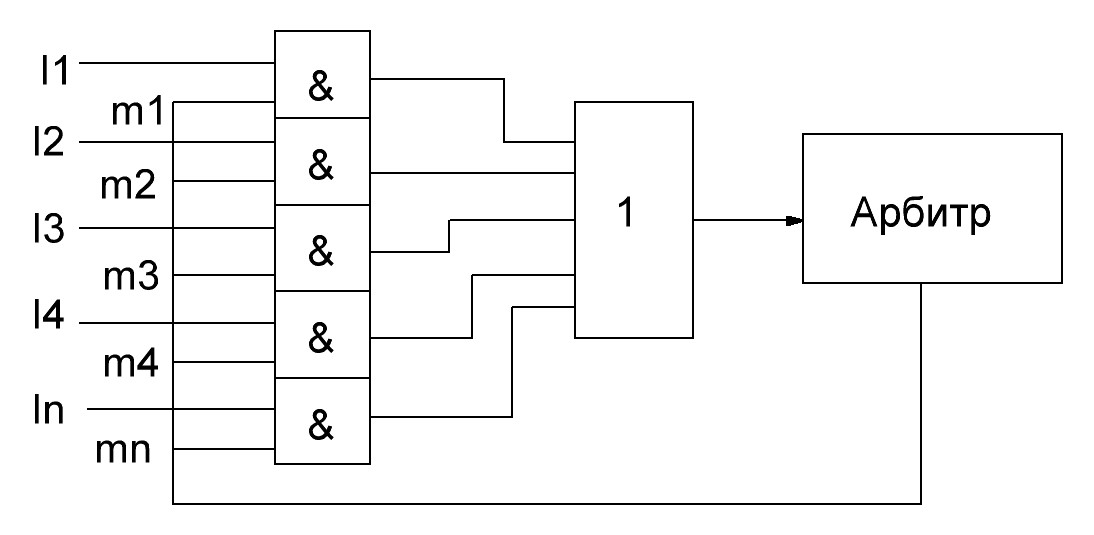
\includegraphics[width=0.8\textwidth]{112_Prosta_cxema.JPG}
\caption{Простейшая схема прерываний с маской}
\end{figure}

Можно выделить две дисциплины обслуживания прерываний: с \textit{относительным} приоритетом и \textit{абсолютным} приоритетом.

В первом случае приоритет сигналов между собой относителен, и рассматривается только в момент одновременного поступления сигналов прерывания, т.е. если сигнал с большим приоритетом поступит позднее сигнала с меньшим приоритетом, то обслуживание его начнется только по завершении обслуживания сигнала с меньшим приоритетом.

В схеме с абсолютными приоритетами иначе, ранг приоритетов учитывается всегда, и в случае поступления сигнала с более высоким приоритетом при обработке запроса с меньшим приоритетом, выполнение задачи приостанавливается и начинается обработка запроса с высоким приоритетом.
\begin{figure}[H]
\centering
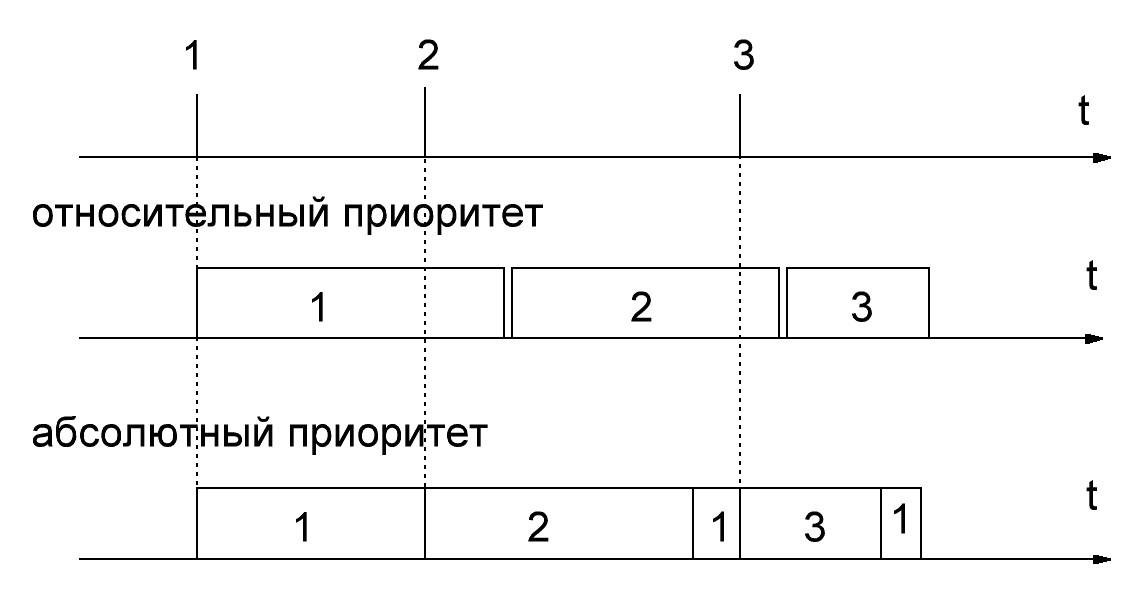
\includegraphics[width=0.8\textwidth]{112_Vrem_prer.JPG}
\caption{Временная диаграмма обслуживания прерываний}
\end{figure}

В зависимости от способов поиска устройств пославших запрос различают следующие структуры прерываний:
\begin{enumerate}
\item С линией запроса

Всякое ВУ способное послать запрос на прерывание имеет специальный сигнал --- сигнал запроса на прерывание. Все эти линии объединены вместе и подключены к входу CPU, требования прерывания. Принцип работы следующий: в некий момент времени одно из ВУ послало запрос на прерывание (в линии прерывания низкий уровень напряжения), устройство пославшее запрос в выходной регистр записывает свой код. CPU получив сигнал запроса должен узнать которое из устройств послало запрос. Для чего CPU выставляет адрес ближайшего ВУ, меньший из всех и читает ШД. Если в устройстве по данному адресу нет кода, то увеличивает значение адреса и читает следующее устройство до получения кода. Этот код назвали вектором прерывания. По вектору прерывания CPU определит начальный адрес подпрограмм обработки этого  запроса. Время реакции на запрос будет различным: у первого ВУ min, у последнего ВУ max. Такое расположение ВУ можно принять за приоритеты и автоматически имеем, что опрашиваем первоначально устройство имеющее высший приоритет.
\begin{figure}[H]
\centering
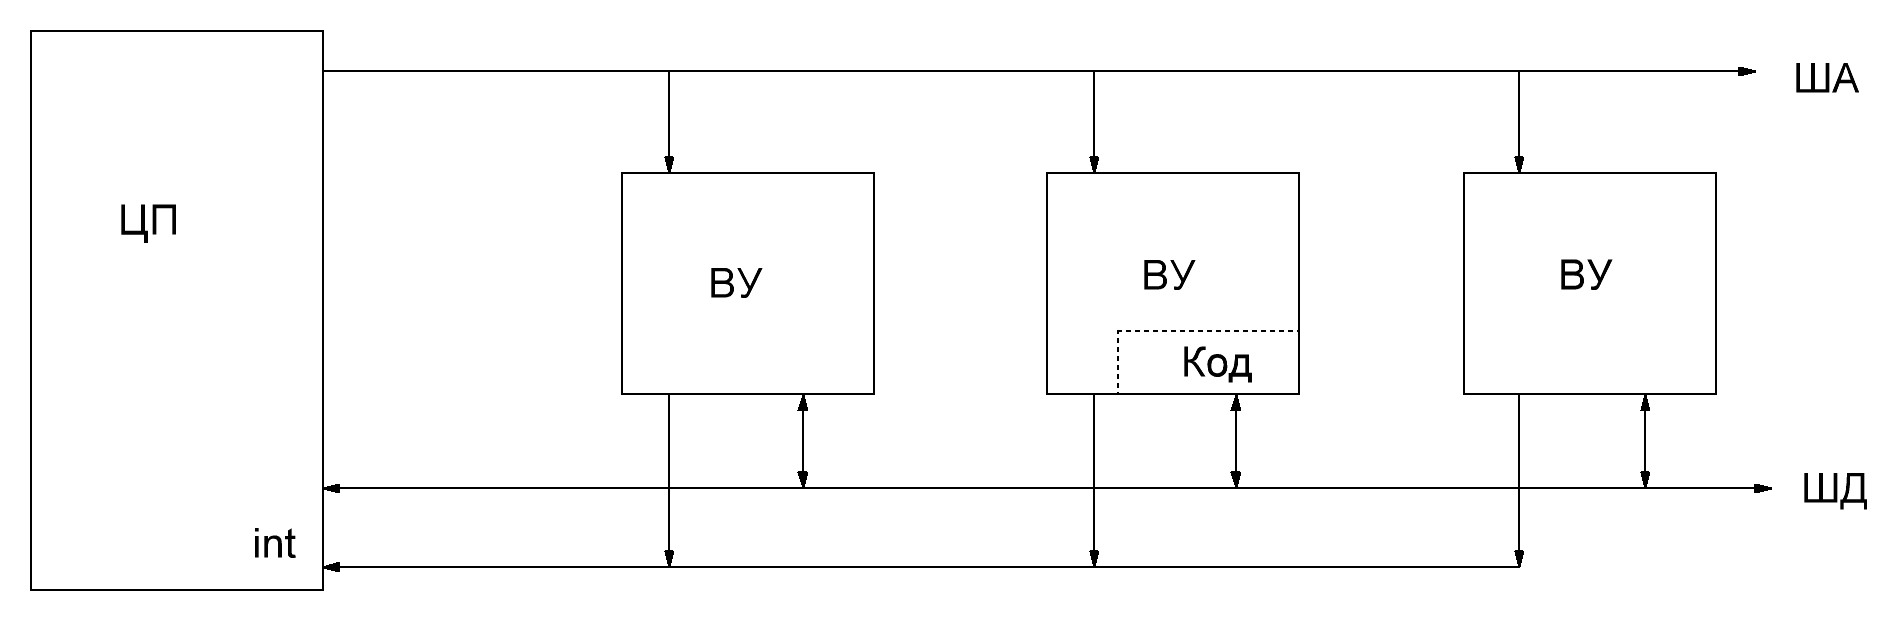
\includegraphics[width=0.8\textwidth]{112_linia_prer.JPG}
\caption{Схема с одной линией прерывания}
\end{figure}

 Главный недостаток подхода время реакции на событие. В тоже время структура проста, требует min оборудования. Для обслуживания такой системы прерываний необходима подпрограмма анализа векторов прерывания. 
\item	Система с линией запроса прерываний и линией подтверждения прерываний. Впервые нашла применение в системе IBM для обслуживания ВУ. Особенность подключения ВУ в том, что каждое имело розетку на блоке канала и вилку у себя и линия подтверждения запроса проходила через все розетки канала к которым можно было бы подключить ВУ. Отличие от 1-ой структуры в том, что опознавание ВУ пославшего запрос выполняется не программно, а аппаратно. CPU по линии подтверждения посылает высокий уровень который проходит через все розетки ВУ. Если ВУ не послало запрос, оно ретранслирует --- передает этот уровень дальше, если послало, ВУ выставляет на ШД вектор прерываний и CPU обращается к подпрограмме обработки по этому вектору. При отсутствии ВУ розетка свободна --- обязательно ставили заглушку, ответную часть разъема с перемычкой по которой сигнал подтверждения передавался дальше.
\begin{figure}[H]
\centering
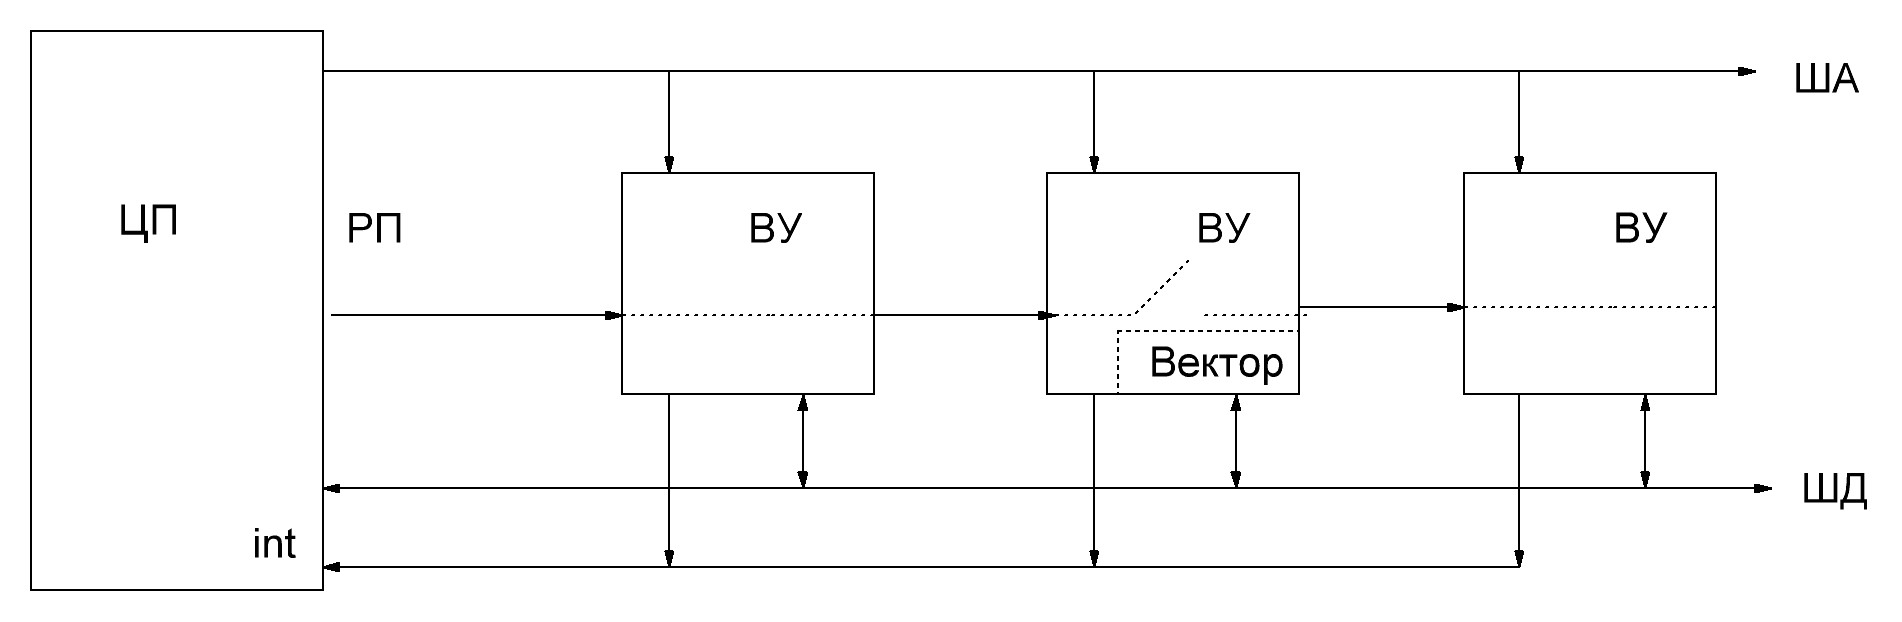
\includegraphics[width=0.8\textwidth]{112_SRP.JPG}
\caption{Схема с разрешением прерывания}
\end{figure}

 Время анализа устройства пославшего запрос небольшое, но само устройство инициирует вектор и соответственно CPU должен иметь подпрограмму анализа вектора прерываний. Что привело к появлению третьих структур: с контроллером прерываний. Последние функции CPU вынесены в дополнительную внешнюю схему называемую контроллером прерываний.
\item	С контроллером прерываний.
В этой структуре адрес устройства, пославшего сигнал прерывания, определяет специальная схема -- контроллер прерываний.

С появлением на любом входе контроллера активного сигнала схема преобразует этот сигнал в адрес входа в подпрограмму прерываний и выставляет его на ШД.

Эта структура наиболее удобна и имеет минимальное время срабатывания. Контроллер прерываний может быть как отдельной схемой, так и быть интегрированным в микропроцессор.

Основные задачи контроллера:
\begin{enumerate}
\item Корректно изменить последовательность вычислений;
\item определить приоритеты;
\item корректно вернуться в прерванную программу;
\end{enumerate}

Последовательность выполнения процедуры прерывания: получение запроса на прерывание от ВУ --> контроллер посылает к ЦП сигнал  прерывания --> контроллер получает подтверждение запроса от ЦП --> контроллер выставляет на ШД вектор прерывания.
\begin{figure}[H]
\centering
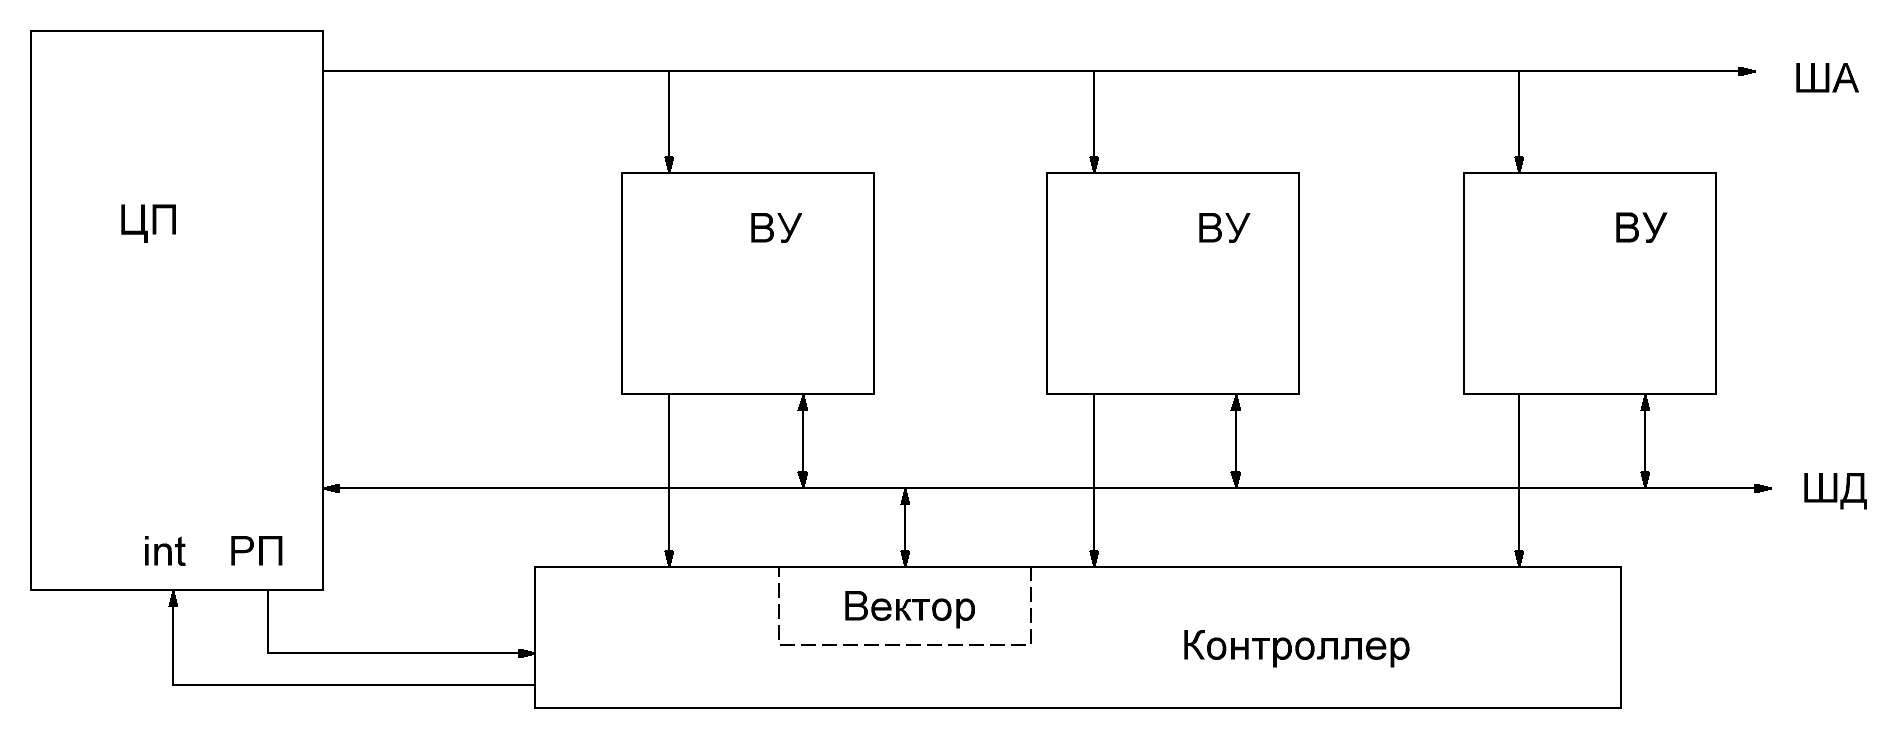
\includegraphics[width=0.8\textwidth]{112_Kontroller.JPG}
\caption{Схема с контроллером прерываний}
\end{figure}

Контроллер, получив сигнал запроса от ВУ(если несколько , то вектор прерывания выбирает по приоритету), выставляет маску на входы прерывания от ВУ. Маскируются только те входы приоритет которых ниже приоритета данного запроса. Посылает запрос на прерывание в ЦП и ждет разрешения прерывания, после получения разрешения прерывания выставляет на ШД вектор прерывания соответствующий ВУ, которое инициализировало запрос.

Если в процессе обработки запроса приходит ещё один запрос на прерывание, то он запоминается контроллером(если его приоритет ниже выполняемого), а затем по окончании выполнения предыдущего запроса инициализируется выполнение следующего запроса.
\end{enumerate}	

Пример распознавания прерывания.
В момент когда приходит один из дискретных сигналов (допустим у нас всего их 8 ), формируется сигнал прерывания для ЦП и начинается обработка прерывания. Для того чтобы узнать какой именно из  8 дискретных побудил прерывание , в момент появления дискретного сигнала состояние всех 8ми записывается в регистр, и затем при обработке прерывания читается из него. Прочитав состояние дискретных входов, ЦП ищет в каком из них активный сигнал (высокий уровень), для этого  производится операция "И" и лог 1 с каждым из битов по очереди, в том где после логического умножения останется 1 и будет нужный нам. 

% Вопрос 113 --------------------------------------------------------
\section{Системы памяти ЭВМ. Назначение каждого типа элементов памяти и место его в иерархии. Что дает для характеристик ЭВМ каждый тип элементов памяти.}

Иерархия памяти строится на основе положения различных устройств памяти относительно АЛУ процессора. Чем ближе устройство памяти к АЛУ, тем короче время доступа к ячейке.

\begin{figure}[H]
\centering
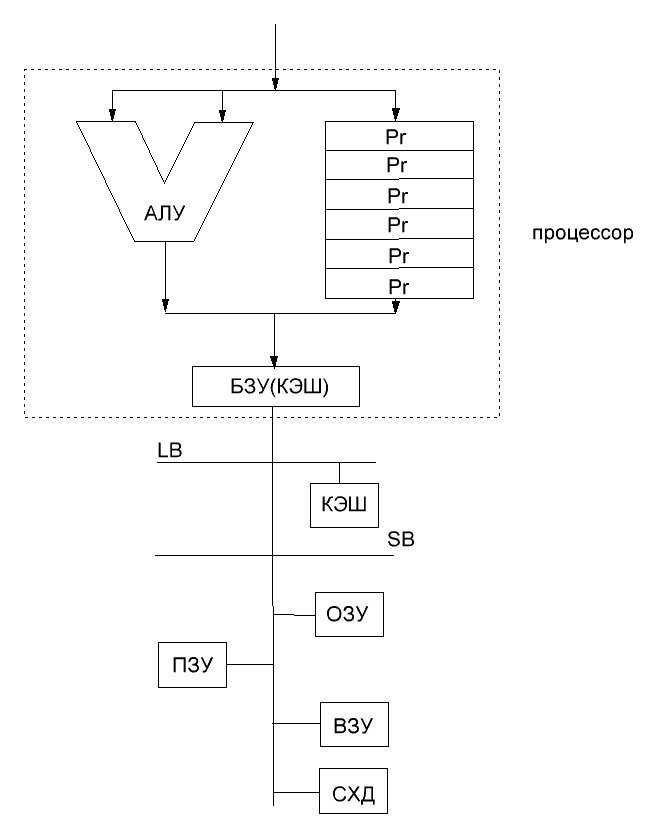
\includegraphics[width=0.8\textwidth]{113_struct.JPG}
\caption{Иерархия памяти ЭВМ}
\end{figure}

Представленное расслоение памяти показывает, что в современной ЭВМ, в отличии от типовой Фон-Неймана память различается по различной степени иерархии в зависимости от быстродействия и объема. Самая быстрая паямть --- регистры процессора(СОЗУ). Число регистров небольшое, назначение --- хранить постоянно необходимую информацию и текущий результат команды. Помимо данных регистры процессора так же хранят адреса сегментов, смещения, текущее состояние счетчиков команд. Непосредственно данных в регистрах до 4 --- 8 слов. Время смены состояния регистров --- от 1 до нескольких тактов. Доступ к регистрам --- в командах процессора.

Вместе с регистрами на кристалле процессора размещают буферное ЗУ-КЭШ. Структура КЭШ так же основана на основе регистров, но эти регистры имеют большую длину --- до 128 слов, и включены по схеме сдвига. Буферные ЗУ по логике включения являются необязательной. Цель --- сократить время доступа процессора к памяти. В некоторых типах микропроцессорах БЗУ отсутствует и при построении вычислительной машины, можно выполнить отдельный модуль БЗУ или КЭШ подключив к локальной шине. При организации ЭВМ, КЭШ может быть один, два на процессоре и локальной шине. КЭШ на процессоре необходим для хранения данных так и кодов команд

Основная память(ОЗУ) через системную магистраль SB соединяется с БЗУ, при этом адреса формируемые процессором, контроллер ОЗУ использует для чтения/записи файлов. Читаем/пишем в ОЗУ не слово, а файлы конечной длины. Поэтому процессор определяет начало и конец файла. В современных ОЗУ разделяют 3 области памяти на всякую задачу: память данных, паямть команд, стэк. Замечательное качеством ОЗУ является малое время чтения/записи, поэтому процессор "не простаивает" обращаясь к памяти. Однако при выключении питания, содержимое ОЗУ исчезает. Поэтому коды команд, библиотеки, результаты вычислений нужно хранить, чтобы использовать второй и следующие разы. С этой целью имеют два устройства: ПЗУ и ВЗУ.

ПЗУ --- память команд. Поскольку сегодня память команд может составлять большие объемы, хранить все в интегральных схемах ПЗУ не имеет смысла. ПЗУ хранит основные управляющие коды для сохранения работоспособности ЭВМ. Это работа С внешними устройствами, загрузчик, постоянные константы. Содержимое ПЗУ пользователь не должен изменять. Мы только читаем то, что там записано.

Системные программы, драйвера внешних устройств не обязательные для минимальной конфигурации ЭВМ храним в ВЗУ.
 
% Вопрос 114 --------------------------------------------------------
\section{Память программ. Виды носителей. Жесткие диски и их твердотельные аналоги.}

Для хранения программ и данных в ЭВМ используют различного рода накопителей, общая емкость которых, как правило в сотни раза превышает емкость оперативной памяти.

По способу записи/чтения информации на носитель,дисковые накопители можно разделить на магнитные, оптические и магнитооптические. Среди дисковых накопителей можно выделить:
\begin{enumerate}
\item накопители на флоппи дисках
\item накопители на несменных жестких дисках
\item накопители на сменных жестких дисках
\item накопители на магнитооптических дисках
\item накопители на оптических компакт дисках
\end{enumerate}

{\it Накопители на жестких магнитных дисках.}

Накопители на жестких магнитных дисках объединяют в одном корпусе носитель (носители) и устройство чтения/записи, а также, нередко, и интерфейсную часть, называемую контроллером жесткого диска. Типичной конструкцией жесткого диска является исполнение в виде одного устройства --- камеры, внутри которой находится один или более дисковых носителей, помещённых на одну ось, и блок головок чтения/записи с их общим приводящим механизмом. Обычно, рядом с камерой носителей и головок располагаются схемы управления головками, дисками и, часто, интерфейсная часть и (или) контроллер. На интерфейсной карте устройства располагается собственно интерфейс дискового устройства, а контроллер с его интерфейсом располагается на самом устройстве. С интерфейсным адаптером схемы накопителя соединяются при помощи комплекта шлейфов.
В отличие от «гибкого» диска (дискеты), информация в НЖМД записывается на жёсткие (алюминиевые или стеклянные) пластины, покрытые слоем ферромагнитного материала.Технология магнитных запоминающих устройств состоит в намагничивании переменным магнитным полем участков носителя и считывания информации, закодированной как области переменной намагниченности. Дисковые носители, как правило, намагничиваются вдоль концентрических полей --- дорожек, расположенных по всей плоскости дискоидального вращающегося носителя. Запись производится в цифровом коде. Намагничивание достигается за счет создания переменного магнитного поля при помощи головок чтения/записи. Головки представляют собой два или более магнитных управляемых контура с сердечниками, на обмотки которых подается переменное напряжение. Изменение величины напряжения вызывает изменение направления линий магнитной индукции магнитного поля и, при намагничивании носителя, означает смену значения бита информации с 1 на 0 или с 0 на 1.
Ёмкость современных жёстких дисков достигает 4000 Гб (4 терабайт) и близится к 5 Тб.

{\it Твердотельные аналоги жесткого диска.}

Твердотéльный накопитель (SSD) --- немеханическое запоминающее устройство на основе микросхем памяти. Кроме них, SSD содержит управляющий контроллер.Различают два вида твердотельных накопителей: SSD на основе памяти, подобной оперативной памяти компьютеров, и SSD на основе флеш-памяти. В настоящее время твердотельные накопители используются в компактных устройствах: ноутбуках, нетбуках, коммуникаторах и смартфонах.

Преимущества:
\begin{enumerate}
\item высокая скорость чтения любого блока данных не зависимо физического от расположения;
\item низкое энергопотребление при чтении данных с накопителя;
\item пониженное тепловыделение;
\item бесшумность и высокая механическая надёжность.
\end{enumerate}

Недостатки: 

\begin{enumerate}
\item высокое энергопотребление при записи блоков данных, энергопотребление растёт с ростом объёма накопителя и интенсивностью изменения данных; 
\item низкая ёмкость и высокая стоимость за гигабайт по сравнению с HDD;
\item ограниченное число циклов записи.
\end{enumerate}

% Вопрос 115 --------------------------------------------------------
\section{Компиляторы. Назначение компиляторов, их виды. Последовательность процедуры компиляции.}

Компилятор --- программа, выполняющая трансляцию исходного кода, написанного на языке высокого уровня, в эквивалентную программу на низкоуровневом языке, близком машинному коду.

Любой компилятор, как программа должен выполнять три обязательные процедуры:
\begin{itemize}
\item Лексический анализ.
\item Синтаксический анализ.
\item Генерация машинных кодов.
\end{itemize}

Основная задача лексического анализа --- разбить входной текст, состоящий из последовательности одиночных символов, на последовательность слов, или лексем, т.е. выделить эти слова из непрерывной последовательности символов. Все символы входной последовательности с этой точки зрения разделяются на символы, принадлежащие каким-либо лексемам, и символы, разделяющие лексемы (разделители). Обычно все лексемы делятся на классы. Примерами таких классов являются числа (целые, восьмеричные, шестнадцатиричные, действительные и т.д.), идентификаторы, строки. Отдельно выделяются ключевые слова и символы пунктуации (иногда их называют символы-ограничители).

Задача синтаксического анализатора --- провести разбор текста программы, сопоставив его с эталоном, данным в описании языка. Синтаксический анализатор (парсер) --- это программа или часть программы, выполняющая синтаксический анализ. При парсинге исходный текст преобразуется в структуру данных, обычно --- в дерево, которое отражает синтаксическую структуру входной последовательности и хорошо подходит для дальнейшей обработки. Как правило, результатом синтаксического анализа является синтаксическая структура предложения, представленная либо в виде дерева зависимостей, либо в виде дерева составляющих, либо в виде некоторой комбинации первого и второго способов представления.

Кодогенерация --- часть процесса компиляции, когда специальная часть компилятора, кодогенератор, конвертирует синтаксически корректную программу в последовательность инструкций, которые могут выполняться на машине. При этом могут применяться различные, в первую очередь машинно-зависимые оптимизации. Часто кодогенератор является общей частью для множества компиляторов, каждый из которых генерирует промежуточный код, который подаётся на вход кодогенератору. Обычно, на вход генератора кода подаётся дерево разбора или абстрактное синтаксическое дерево. Дерево преобразуется в линейную последовательность инструкций промежуточного языка (например, в трехадресный код).

Виды компиляторов:

\begin{itemize}
\item Векторизующий. Транслирует исходный код в машинный код компьютеров, оснащённых векторным процессором.
\item Гибкий. Сконструирован по модульному принципу, управляется таблицами и запрограммирован на языке  высокого уровня или реализован с помощью компилятора компиляторов.
\item Инкрементальный. Повторно транслирует фрагменты программы и дополнения к ней без перекомпиляции всей программы.
\item Интерпретирующий (пошаговый). Последовательно выполняет независимую компиляцию каждого отдельного оператора (команды) исходной программы.
\item Отладочный. Устраняет отдельные виды синтаксических ошибок.
\item Резидентный. Постоянно находится в оперативной памяти и доступен для повторного использования многими задачами.
\item Самокомпилируемый. Написан на том же языке, с которого осуществляется трансляция.
\item Универсальный. Основан на формальном описании синтаксиса и семантики входного языка. Составными частями такого компилятора являются: ядро, синтаксический и семантический загрузчики.
\end{itemize}

% Вопрос 116 --------------------------------------------------------
\section{Контроль информации при последовательной передаче двоичного кода. Методы контроля. Контроль передачи информации при обмене словами (байтами). Методы.}

Считается, что цифровая техника обеспечивает безошибочные вычисления, так как информация представлена однозначно в виде 0 и 1, в отличие от аналоговых схем, где носителем информации является уровень сигнала, который может меняться. Однако, при передаче и хранении информации возможно ее искажение, поэтому вводятся средства контроля, цель которых --- не остановить вычисления, а получить результат с максимальной достоверностью.

Контроль проводится как аппаратными средствами, так и программными. Аппаратные средства включаются в состав функциональных блоков процессора, контроллера ввода/вывода, средств передачи. Программно контролируются память, выполнение отдельных операций.
Назначение всех средств контроля можно разделить на контроль передачи информации и контроль преобразования.

\begin{center}
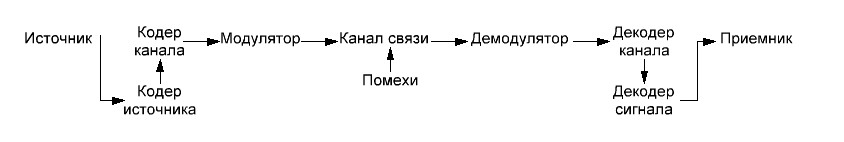
\includegraphics[width=0.9\textwidth]{116_Channel.png}
\end{center}

Для повышения помехоустойчивости к передаваемому коду добавляют доп. разряды, при этом число возможных состояний кода увеличивается, однако число информативных состояний остается прежним. То есть часть состояний --- запрещенные. Кодовое расстояние --- число разрядов из всей совокупности передаваемых кодов, в которых 1 и 0 не совпадают.

Простейшие коды:
\begin{enumerate}
\item добавление контрольного разряда --- контроль четности. Двойные ошибки не замечаются, исправление информации невозможно --- только контроль правильности.
\item Коды Хэмминга. Кодовое расстояние --- 3. Позволяют выявить и исправить одиночную ошибку. Получаются путем объединения по XOR части разрядов числа, но несколько раз.
\item Простой повтор нечетное число раз --- по большинству.
\end{enumerate}

При передаче файлами применяется контроль с помощью СRC-кода. Суть: после передачи файла к нему прицепляется контрольная последовательность, получаемая как остаток от деления значения файла на определенный полином, известный и приемнику, и источнику. Полином выбран так, что его значение в квадрате меньше максимального значения файла. Приемник, зная полином, вычисляет свой CRC и сравнивает его с полученным от источника. Если совпадают --- передача правильная. Если нет --- запрашивается повтор передачи.

Метод наибольшего правдоподобия --- по алгоритму Виттерби. Он при приеме предусматривает некоторые ожидаемые стандартные комбинации. В настоящее время применяется в системах цифровой связи.

% Вопрос 117 ----------------------------------------------------------
\section{Приведите основные структуры объединения процессоров в многопроцессорных системах. В чем суть ограничений архитектуры Фон-Неймана.}

Для архитектуры фон Неймана характерны следующие свойства:
\begin{enumerate}
\item единый процессор и единая память
\item линейная организация памяти
\item команды низкого уровня
\item любая операция предусматривает чтение памяти команд, и только затем --- обращение к памяти данных. Связь процессора с памятью по ША и ШД.
\end{enumerate}

Реальные проводники из-за своих паразитных характеристик не позволяют передавать сигналы с высокой скоростью, поэтому увеличение производительности за счет повышения тактовой частоты уже почти невозможно. Таким образом, нужны новые структуры ЭВМ.
\begin{enumerate}
\item конвейерная --- ряд процессоров, специализированных под конкретные операции, выполняют операции последовательно, передавая результат друг другу. За счет этого может выполняться одновременное преобразование нескольких слов данных. Конвейер реализуется на кристалле, т.к. отдельные блоки объединять накладно.
\item параллельная --- объединение нескольких машин через канал. Канал --- узкое место. Например, двухмашинный комплекс, в котором вторая машина работает в качестве горячего резерва.
\item иерархическая --- один из процессоров выделяется как главный, вспомогательный подключается через блок сопряжения, но при этом теряется универсальность.
\end{enumerate}

Векторно-конвейерные суперкомпьютеры. Конвейер, как последовательное включение процессорных блоков, сохраняется, однако каждый процессорный блок обрабатывает не одно слово данных, а вектор --- несколько составленных вместе слов, т.е. в структуре ЭВМ имеются параллельные каналы обработки, соединенные в конвейер. Основная идея --- распараллеливание циклического процесса.

Симметричные (SMP) системы --- системы с общей памятью. Подключение нескольких процессоров к общей памяти, каждому процессору выделяется буферная память. При этом пока один процессор занимает шину, остальные могут работать с информацией из кэша. С ростом числа процессоров эффективность метода падает, т.к. приходится постоянно наполнять кэш. Замена шины на электронный коммутатор позволяет увеличить скорость передачи и организовать уже несколько одновременных процессов обращения к памяти. 

Структуры с массовым параллелизмом (MPP) --- предельный случай SMP, когда каждому процессору выделен свой блок памяти. В структуре те же блоки, но компоновка иная. Например, обмен информацией происходит по пути: память 1 -> кэш 1-го проц. -> коммутатор -> кэш 2-го проц. -> память 2. Раздельная память увеличивает интенсивность обмена процессора со своей памятью, и лишь малое время уходит на обмен между блоками памяти разных процессоров, как правило --- после выполнения каких-либо законченных процедур.

\begin{center}
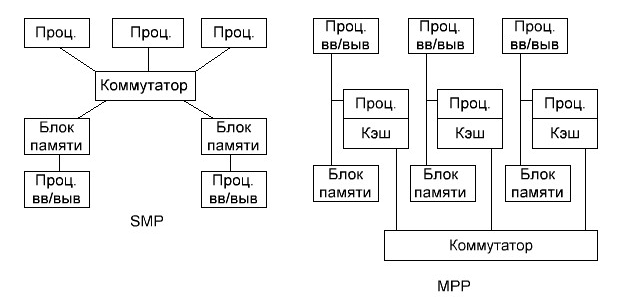
\includegraphics[width=0.8\textwidth]{117_SMP_MPP.png}
\end{center}
Кластеры --- объединение в единое вычислительное пространство самостоятельных ВС по быстрым сетям. В кластере должен быть управляющий блок --- аналог сетевого сервера, по скорости значительно превосходящий остальные узлы. Его задача --- распределение и контроль информации.

% Вопрос 118 ----------------------------------------------------------
\section{Сравните структуры двух МПК, имеющих организацию SMP и MPP. Приведите их структурные схемы.}

Симметричные (SMP) системы --- системы с общей памятью. Подключение нескольких процессоров к общей памяти требует подключения их к общим шинам адреса и данных. При параллельном подключении процессоров к шине доступ к памяти разрешен только одному --- это не увеличивает производительность, поэтому каждому процессору выделяется буферная память. При этом пока один процессор занимает шину, остальные могут работать с информацией из кэша. С ростом числа процессоров эффективность метода падает, т.к. приходится постоянно наполнять кэш. Замена шины на электронный коммутатор позволяет увеличить скорость передачи и организовать уже несколько одновременных процессов обращения к памяти. Адресное пространство для всех общее, но оно распределено по некольким модулям. Каждый процессор преимущественно работает со своим модулем, но может обратиться и к любому другому. Внешние устройства подключаются к блоку памяти или коммутатору через специальные каналы --- процессоры ввода/вывода.

Пример SMP системы --- "МВК Эльбрус". Общее число процессоров --- до 10. Память разделена на 2 логических блока, но адресное пространство общее. Выделяется один управляющий процессор. Развитая система вв\textbackslash выв, так как комплекс должен обслуживать технологическое оборудование.

\begin{center}
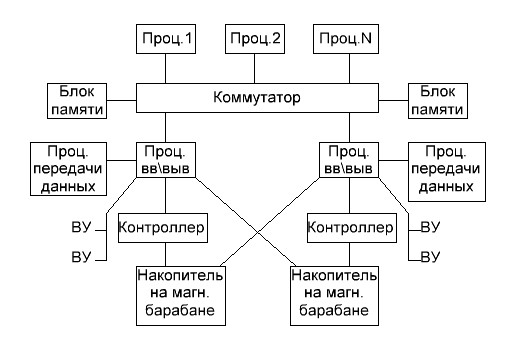
\includegraphics[width=0.7\textwidth]{118_Elbrus.png}
\end{center}
Структуры с массовым параллелизмом (MPP) --- предельный случай SMP, когда каждому процессору выделен свой блок памяти. В структуре те же блоки, но компоновка иная. Например, обмен информацией происходит по пути: память 1 ->кэш 1-го проц.->коммутатор->кэш 2-го проц.-> память 2. Раздельная память увеличивает интенсивность обмена процессора со своей памятью, и лишь малое время уходит на обмен между блоками памяти разных процессоров, как правило --- после выполнения каких-либо законченных процедур.

С ростом числа процессоров растет сложность коммутаторов. Простейшая структура --- матрица. Сложнее --- цилиндр, затем --- тор (он же --- "куб"), соединение кубов --- "гиперкуб".

Пример MPP --- структуры --- МВС-1000. Система 3-го поколения. Размещается в стойках промышленного стандарта. Всего 768 процессоров (по 64 в стойке). В состав системы входят управляющая ЭВМ, файл-сервер, сеть межпроцессорного обмена и FastEthernet. Обязательно --- система контроля питания. Коммутатор --- двумерный тор.

\begin{center}
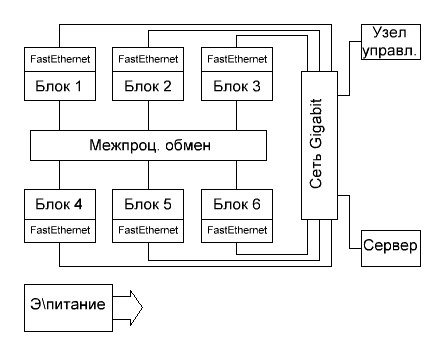
\includegraphics[width=0.7\textwidth]{118_MBC-1000.png}
\end{center}
% Вопрос 119 ----------------------------------------------------------
\section{Сравните характеристики двух последовательных интерфейсов RS-232С и USB. Приведите  структурную организацию интерфейсов и формат передаваемых данных.}

RS-232C --- последовательная передача по байтам. Формат передачи: стартовый сигнал (1,5-2 такта), 8 разрядов данных от младшего к старшему со строго определенной заранее скоростью, затем контрольный разряд, затем стоповый сигнал и небольшая пауза. Скорости: 2400, 4800, 9600, 19200, 38400.

Для двустороннего обмена достаточно трех проводников --- TXD, RXD, GND. Кабель перекручен (TXD источника подключается к RXD приемника, и наоборот). Разъемы COM-порта --- DB-25, DB-9. Помимо информационных сигналов, через разъем посылаются сигналы сопровождения --- ошибка, готовность.

Интерфейс потенциальный, уровни 0 и 1 передаются уровнями напряжения ±5…15 В. Максимальная длина кабеля --- 1,4…1,7 м.

USB --- последовательный цепочечный интерфейс с обменом файлами. Частота --- 33,6 МГц. Сигналы на линиях --- дифференциальные, то есть сигнал распространяется токовый. Размах --- ±4 В при питании 5 В. Интерфейс реализуется микросхемой-адаптером с буферной памятью. Обмен между ней и процессором идет с временем цикла процессора, а передача всегда с фиксированной скоростью, то есть для нее нужен собственный тактовый генератор. Время передачи файла соизмеримо с передачей 1 бита по COM-порту. Плата за  скорость --- аппаратная часть.

Формат кадра:
\begin{itemize}
\item стартовый импульс
\item адресная часть --- 7 бит, адресует до 127 устройств.
\item биты передаваемой информации --- число фиксированное, зависит от принятого формата
\item разряды контроля --- 5-7 бит --- CRC-код.
\item бит конца передачи.
\end{itemize}

Таким образом, передача по кадрам асинхронная, но внутри кадра биты передаются со строго определенной скоростью. В качестве кабеля применяют витую пару (50 Ом). Длина 3…10 м (но рекомендуется не более 5).

% Вопрос 120 ----------------------------------------------------------
\section{Какие принципы программного управления характерны для командного и микро-командного способов управления. В чем сходство и различие этих способов. Покажите на примере структурной схемы устройств управления.}

Принципы программного управления:
\begin{enumerate}
\item Информация кодируется в двоичной форме и разделяется на слова
\item Перед обработкой слова информации исходные данные размещаются в ячейках памяти ЭВМ. Ячейки памяти нумеруются --- адреса.
\item Алгоритм обработки представляется в виде последовательности команд --- программы. Каждая команда задает ЭВМ тип выполняемой операции и может определять местоположение операндов в памяти ЭВМ указанием  номера ячейки.
\item Команды также кодируются в двоичной форме и располагаются в ячейках памяти ЭВМ
\item Выполнение программы сводится к поочередному выбору команд из памяти ЭВМ и их выполнению. Порядок их выполнения задается алгоритмом и зависит от исходных данных
\end{enumerate}

Три уровня команд:
\begin{enumerate}
\item микрокоманды --- элементарное преобразование операнда (пересылка из регистра в регистр, вывод содержимого на выход данных). Микрокоманда выполняется за один такт синхронизации. За время выполнения микрокоманды происходит фиксация входного операнда в регистре процессора (по фронту синхр.) и само преобразование операнда с фиксацией в выходном регистре (по срезу синхр.). Длительность синхросигнала должна быть достаточной для того, чтобы успели закончиться переходные процессы в комбинационных схемах и при записи в регистр.
\item команды --- часто приравнивают к операциям. Команда может включать в себя до десятков микрокоманд.
\item макрокоманды (тэги) --- появились в силу того, что сложные процедуры требовали большого числа команд, обращений в память. Переход к макрокомандам сокращал их число, повышая скорость выполнения.
\end{enumerate}

Устройство управления с жесткими связями.

Процессор с командным типом управления включает в себя управляющую и операционную части. На вход управляющей поступает КОП, который расшифровывается в сигналы микрокоманд. По результатам текущих операций в управляющую часть возвращаются флаги.
Дешифратор команд выполнен на ПЛМ. Сам пользователь не может изменить ее содержимое.

\begin{center}
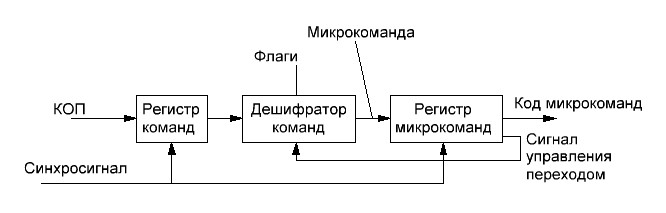
\includegraphics[width=0.8\textwidth]{120_microcom.png}
\end{center}
Устройство микропрограммного управления

В его основе лежит введение промежуточного преобразования кода команд в микрокоманды с применением схем памяти. С приходом КОП дешифратор начального адреса микрокоманды формирует адрес, по которому из памяти микрокоманд необходимо считать первую микрокоманду. Считанный код содержит признак смещения, по которому определяется адрес следующей микрокоманды. Замена содержимого памяти микрокоманд эквивалентна замене микрокоманд. Для анализа текущего состояния процессора на схему управления поступают сигналы управления --- флаги.

\begin{center}
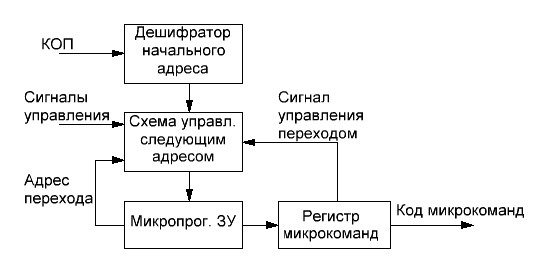
\includegraphics[width=0.8\textwidth]{120_microprog.png}
\end{center}

\end{document}